% ============================================================
%  Visual Localization 2026 --- Technical Report
%  Assignment Solution: Monocular VIO on tbuggy Desert Dataset
%  Author: Udit Singh Parihar
%  Build:  pdflatex assignment_solution.tex
%          (run from colcon_ws_tii/ directory)
% ============================================================
\documentclass[10pt,a4paper]{article}

\usepackage[top=2cm, bottom=2cm, left=2.2cm, right=2.2cm]{geometry}
\usepackage[T1]{fontenc}
\usepackage[utf8]{inputenc}
\usepackage{lmodern}
\usepackage{microtype}
\usepackage{amsmath}
\usepackage{graphicx}
\usepackage{subcaption}
\usepackage{booktabs}
\usepackage{multirow}
\usepackage[table,xcdraw]{xcolor}
\usepackage{listings}
\usepackage[hidelinks,colorlinks=true,linkcolor=blue!70!black,urlcolor=blue!70!black,citecolor=green!50!black]{hyperref}
\usepackage{enumitem}
\usepackage{float}
\usepackage{caption}
\usepackage{parskip}

\graphicspath{{utils/results/}}

% ---------- Code listing style ----------
\definecolor{codebg}{rgb}{0.96,0.96,0.96}
\definecolor{keywordcolor}{rgb}{0.0,0.35,0.65}
\lstset{
  backgroundcolor=\color{codebg},
  basicstyle=\ttfamily\footnotesize,
  keywordstyle=\color{keywordcolor}\bfseries,
  commentstyle=\color{gray},
  stringstyle=\color{orange!70!black},
  breaklines=true,
  frame=single,
  framerule=0.4pt,
  rulecolor=\color{gray!50},
  numbers=none,
  captionpos=b,
  xleftmargin=4pt,
  xrightmargin=4pt,
}

% ---------- Title ----------
\title{%
  \textbf{Visual Localization for a Desert UGV}\\[4pt]
  \large Monocular VIO with OpenVINS on the \textit{tbuggy} Dataset\\[2pt]
  \normalsize Visual Localization 2026 --- Assignment Solution
}
\author{Udit Singh Parihar}
\date{March 2026}

\begin{document}
\maketitle
\vspace{-8pt}
\hrule
\vspace{4pt}

\noindent\textbf{Repository:}
\url{https://github.com/UditSinghParihar/tbuggy_localization}
\hfill
\textbf{Docker image:} \texttt{uditsinghparihar/tbuggy\_vio:latest}

\vspace{2pt}\hrule\vspace{8pt}

\begin{figure}[H]
  \centering
  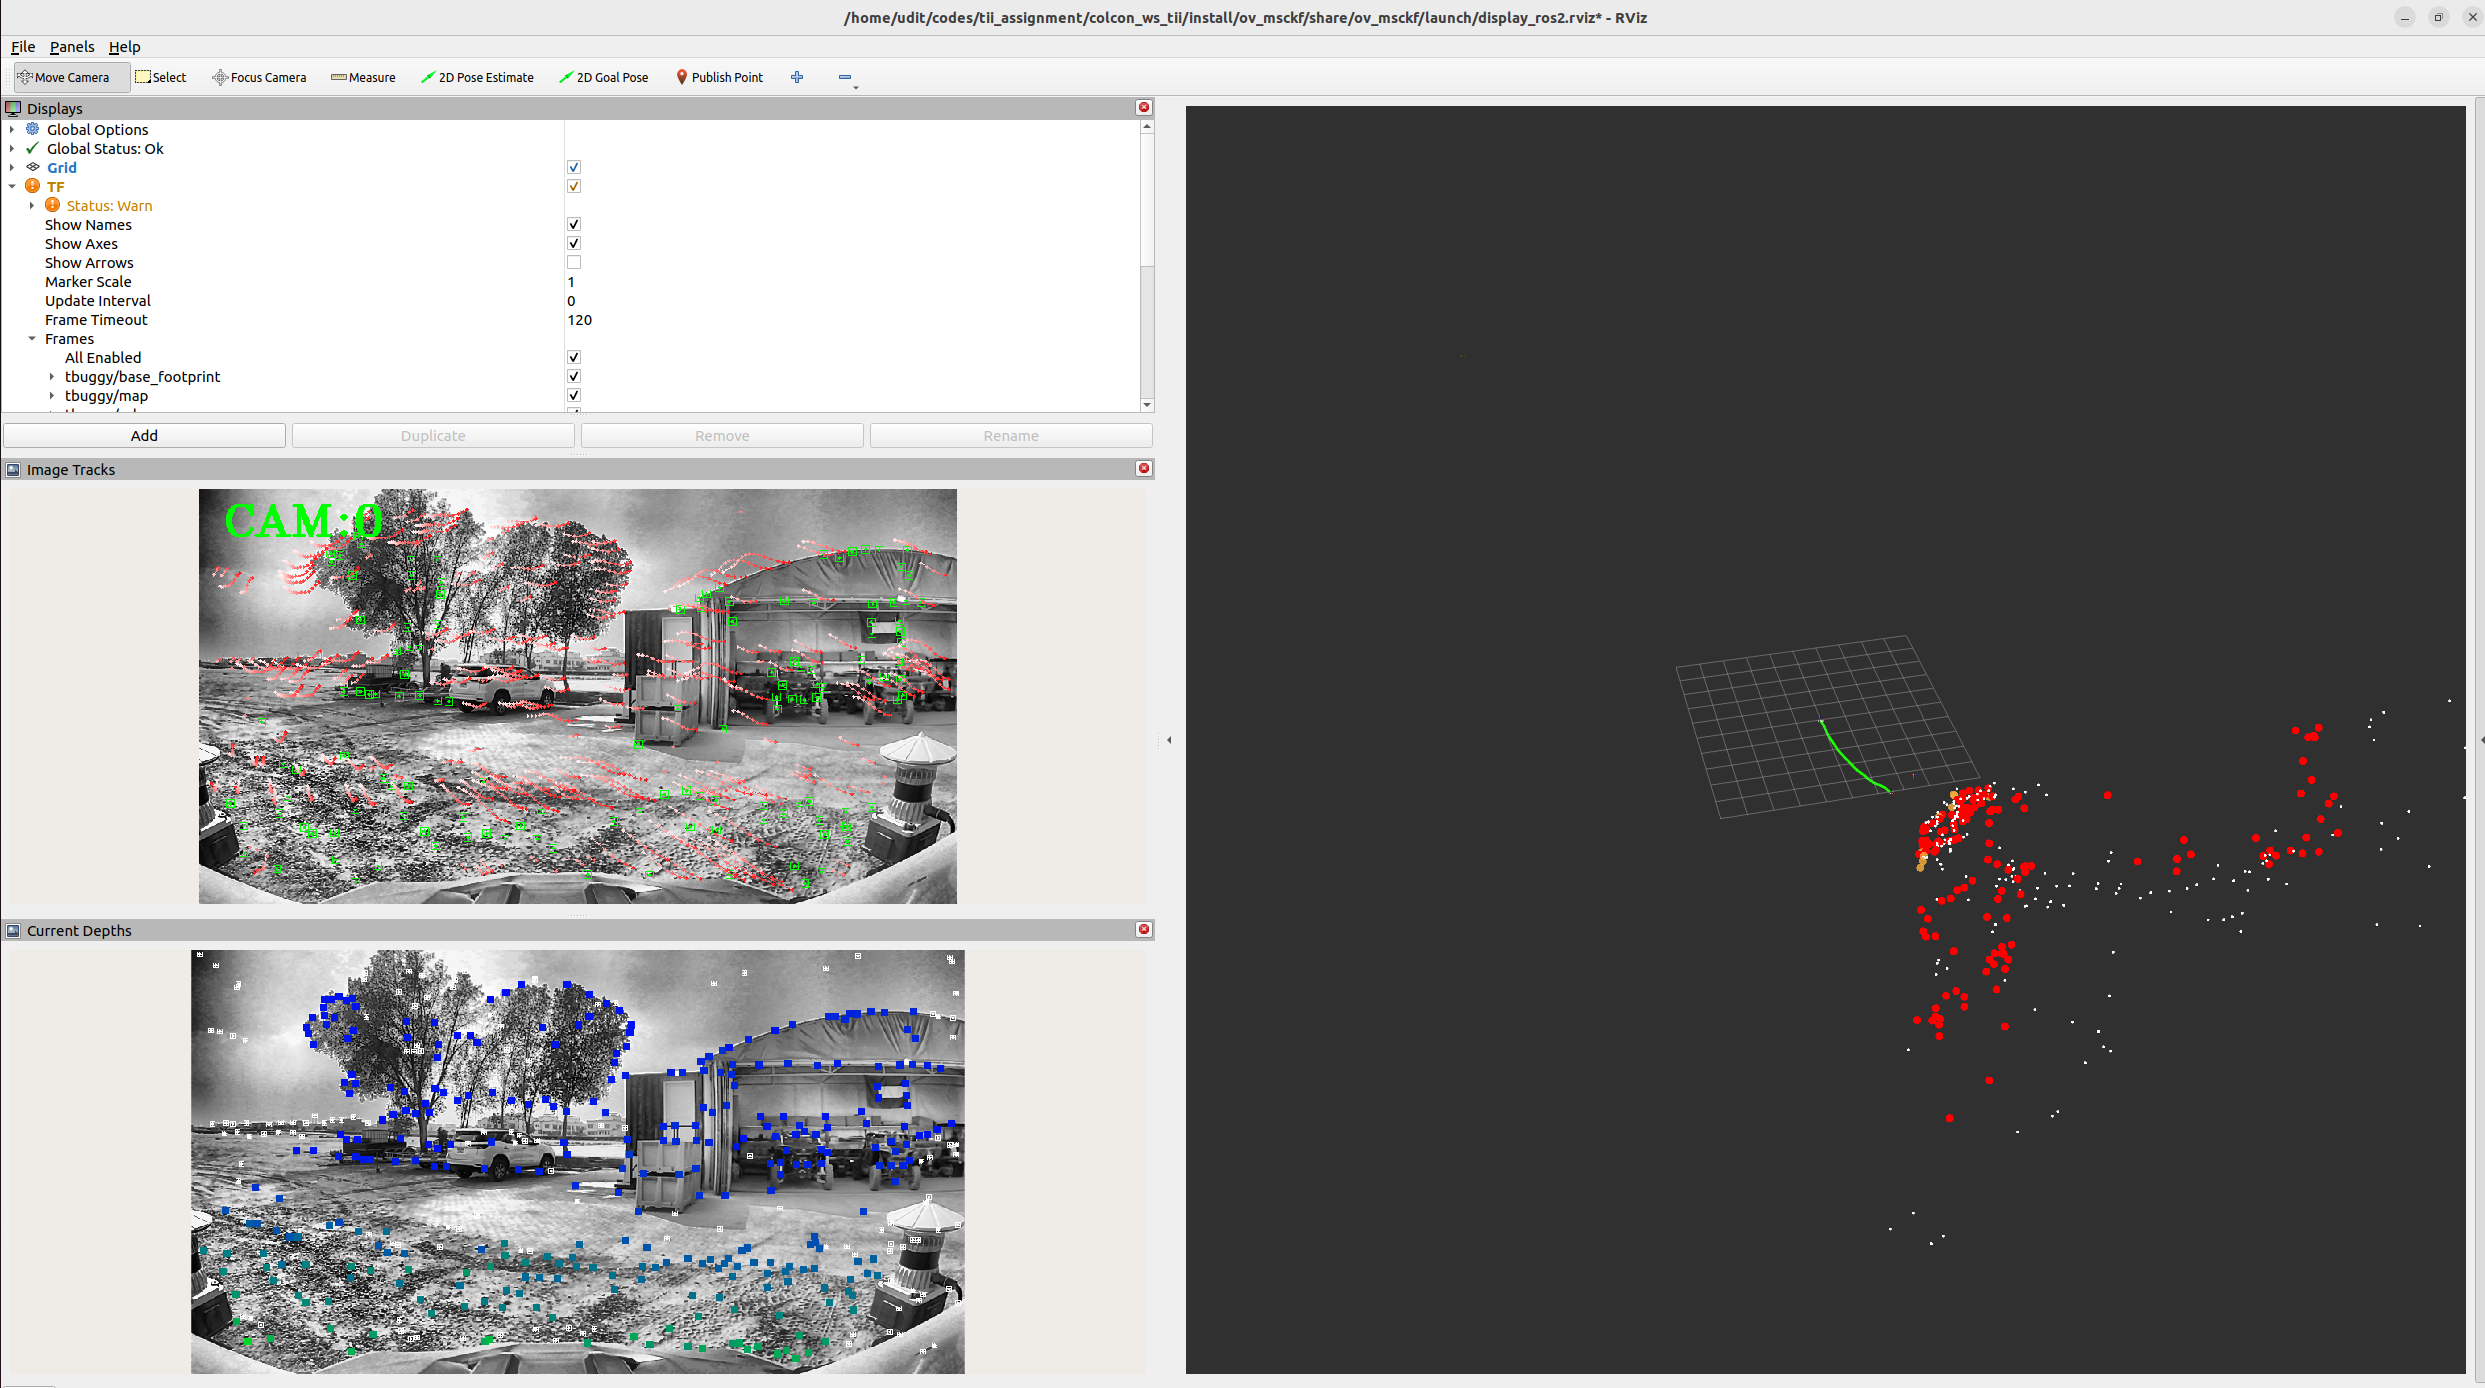
\includegraphics[width=\textwidth]{log_02_start_rviz.png}
  \caption{\textbf{Teaser --- OpenVINS on log\_02, start of sequence.}
  \textit{Left panels:} RViz2 camera views --- top shows KLT feature tracks (red dots = active
  MSCKF features, green lines = track history) on the hangar facade and parked vehicles;
  bottom shows SLAM landmark projections (blue circles) reprojected onto the current frame,
  densely covering the building facade and ground plane.
  \textit{Right panel:} 3D world view at initialisation --- red point cloud is the SLAM landmark
  map already forming from the rich hangar texture; grey grid is the ground plane; short green
  arc is the trajectory so far (vehicle just departed).}
  \label{fig:teaser}
\end{figure}

\noindent\textbf{Abstract.}
We implement a monocular visual-inertial odometry (VIO) pipeline on a desert UGV dataset using
OpenVINS 2.7 (MSCKF). Starting from bag-extracted sensor calibration data, we configure and tune
the estimator across three runs, achieving an Absolute Trajectory Error (ATE) RMSE of
\textbf{41.3\,m over a 1059\,m path (3.9\% error)} on the tuning sequence and \textbf{35.6\,m over 716\,m
(5.0\%)} on a held-out robustness sequence --- without re-tuning. The full pipeline (bag conversion,
GT extraction, OpenVINS launch, evaluation, plots) is containerised in a single Docker image.

% ===========================================================
\section{Data Exploration}
% ===========================================================

\subsection{Dataset Overview}

Two ROS1 bag sequences are provided, converted to ROS2 format for OpenVINS compatibility.

\begin{table}[H]
\centering
\caption{Bag sequence summary}
\begin{tabular}{lrrrrr}
\toprule
Sequence & Duration & Camera frames & IMU msgs & GT odom msgs & GT path length \\
\midrule
log\_01 & 549.8\,s & 16\,473 & 54\,969 & 21\,991 & 1059\,m \\
log\_02 & 336.7\,s & 10\,091 & 33\,648 & 13\,467 &  716\,m \\
\bottomrule
\end{tabular}
\end{table}

\noindent\textbf{Topics used by the pipeline:}
\begin{itemize}[nosep]
  \item \texttt{/tbuggy/camera\_front/image\_raw} --- monocular image stream for feature tracking (1920$\times$1080, $\approx$28\,Hz)
  \item \texttt{/tbuggy/imu\_ins} --- IMU pre-integration; offline noise characterisation for calibration ($\approx$100\,Hz)
  \item \texttt{/tbuggy/odom} --- ground truth for ATE/RPE evaluation ($\approx$40\,Hz)
  \item \texttt{/tf\_static} --- TF chain for camera-IMU extrinsic $\mathbf{T}_{\text{imu,cam}}$
\end{itemize}
\texttt{/tbuggy/fix} (GPS) and \texttt{/tbuggy/relative\_odom} are present in the bag but were \textbf{not used} --- GPS was not needed since \texttt{/tbuggy/odom} provides sufficient ground truth for evaluation.

\subsection{Ground Truth Trajectories}

\begin{figure}[H]
  \centering
  \begin{subfigure}[t]{0.48\textwidth}
    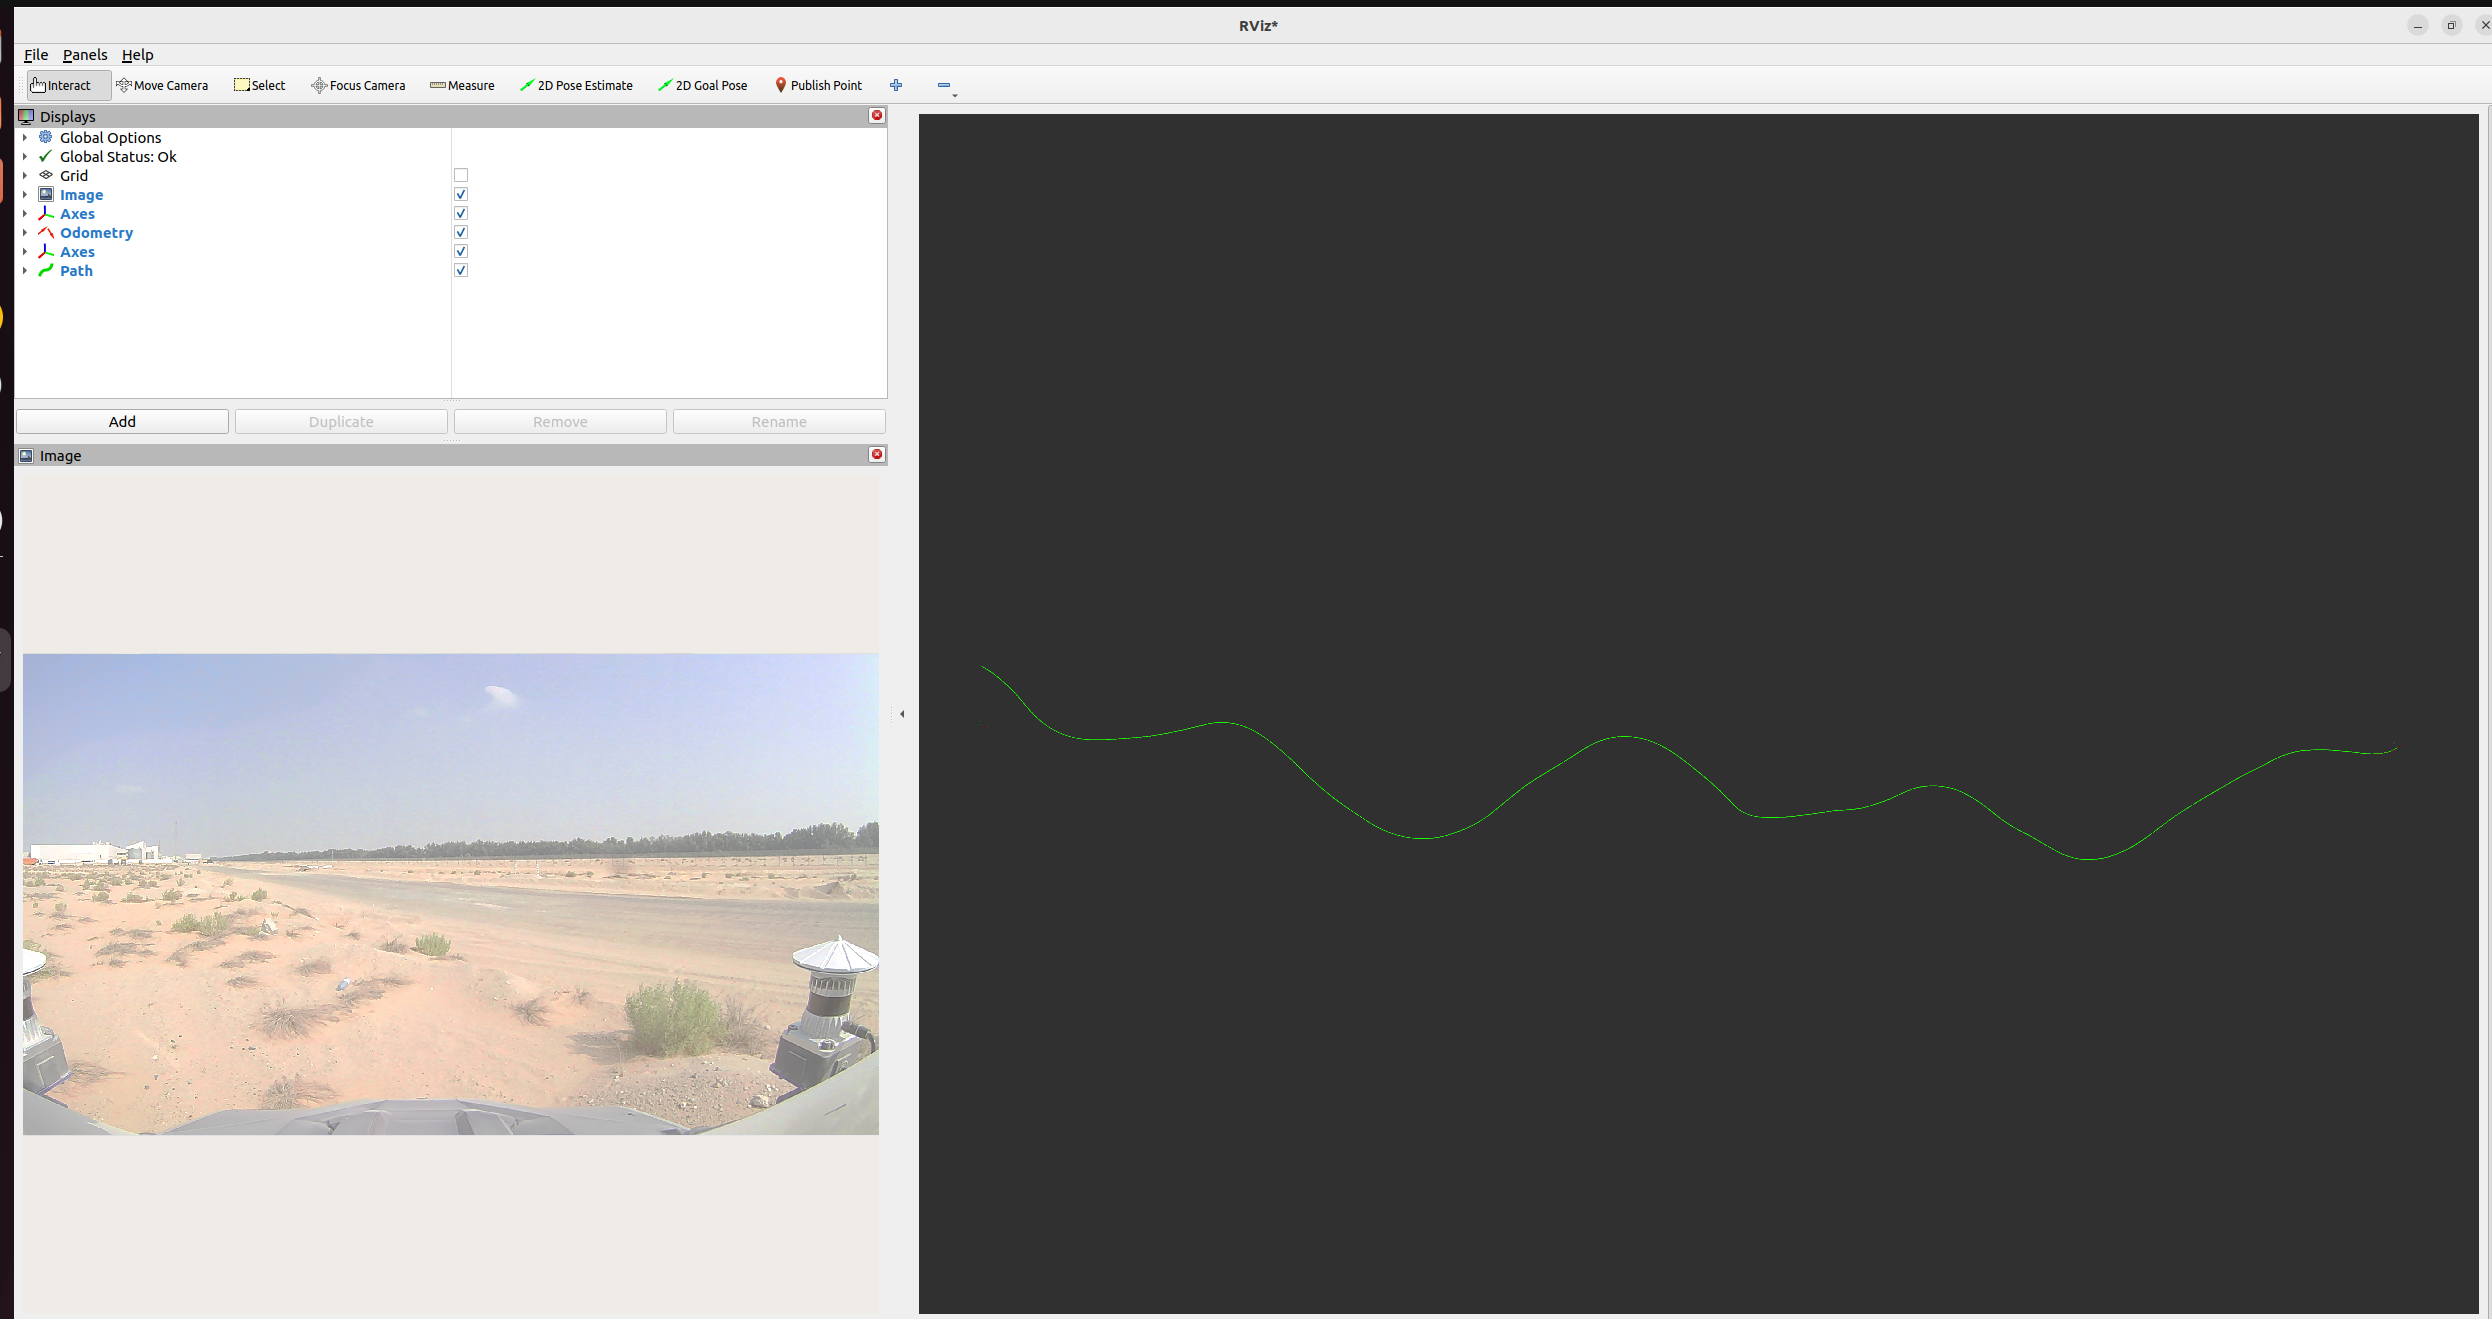
\includegraphics[width=\textwidth]{log01_full_trajectory.png}
    \caption{log\_01: 1059\,m roughly linear desert traverse.}
  \end{subfigure}
  \hfill
  \begin{subfigure}[t]{0.48\textwidth}
    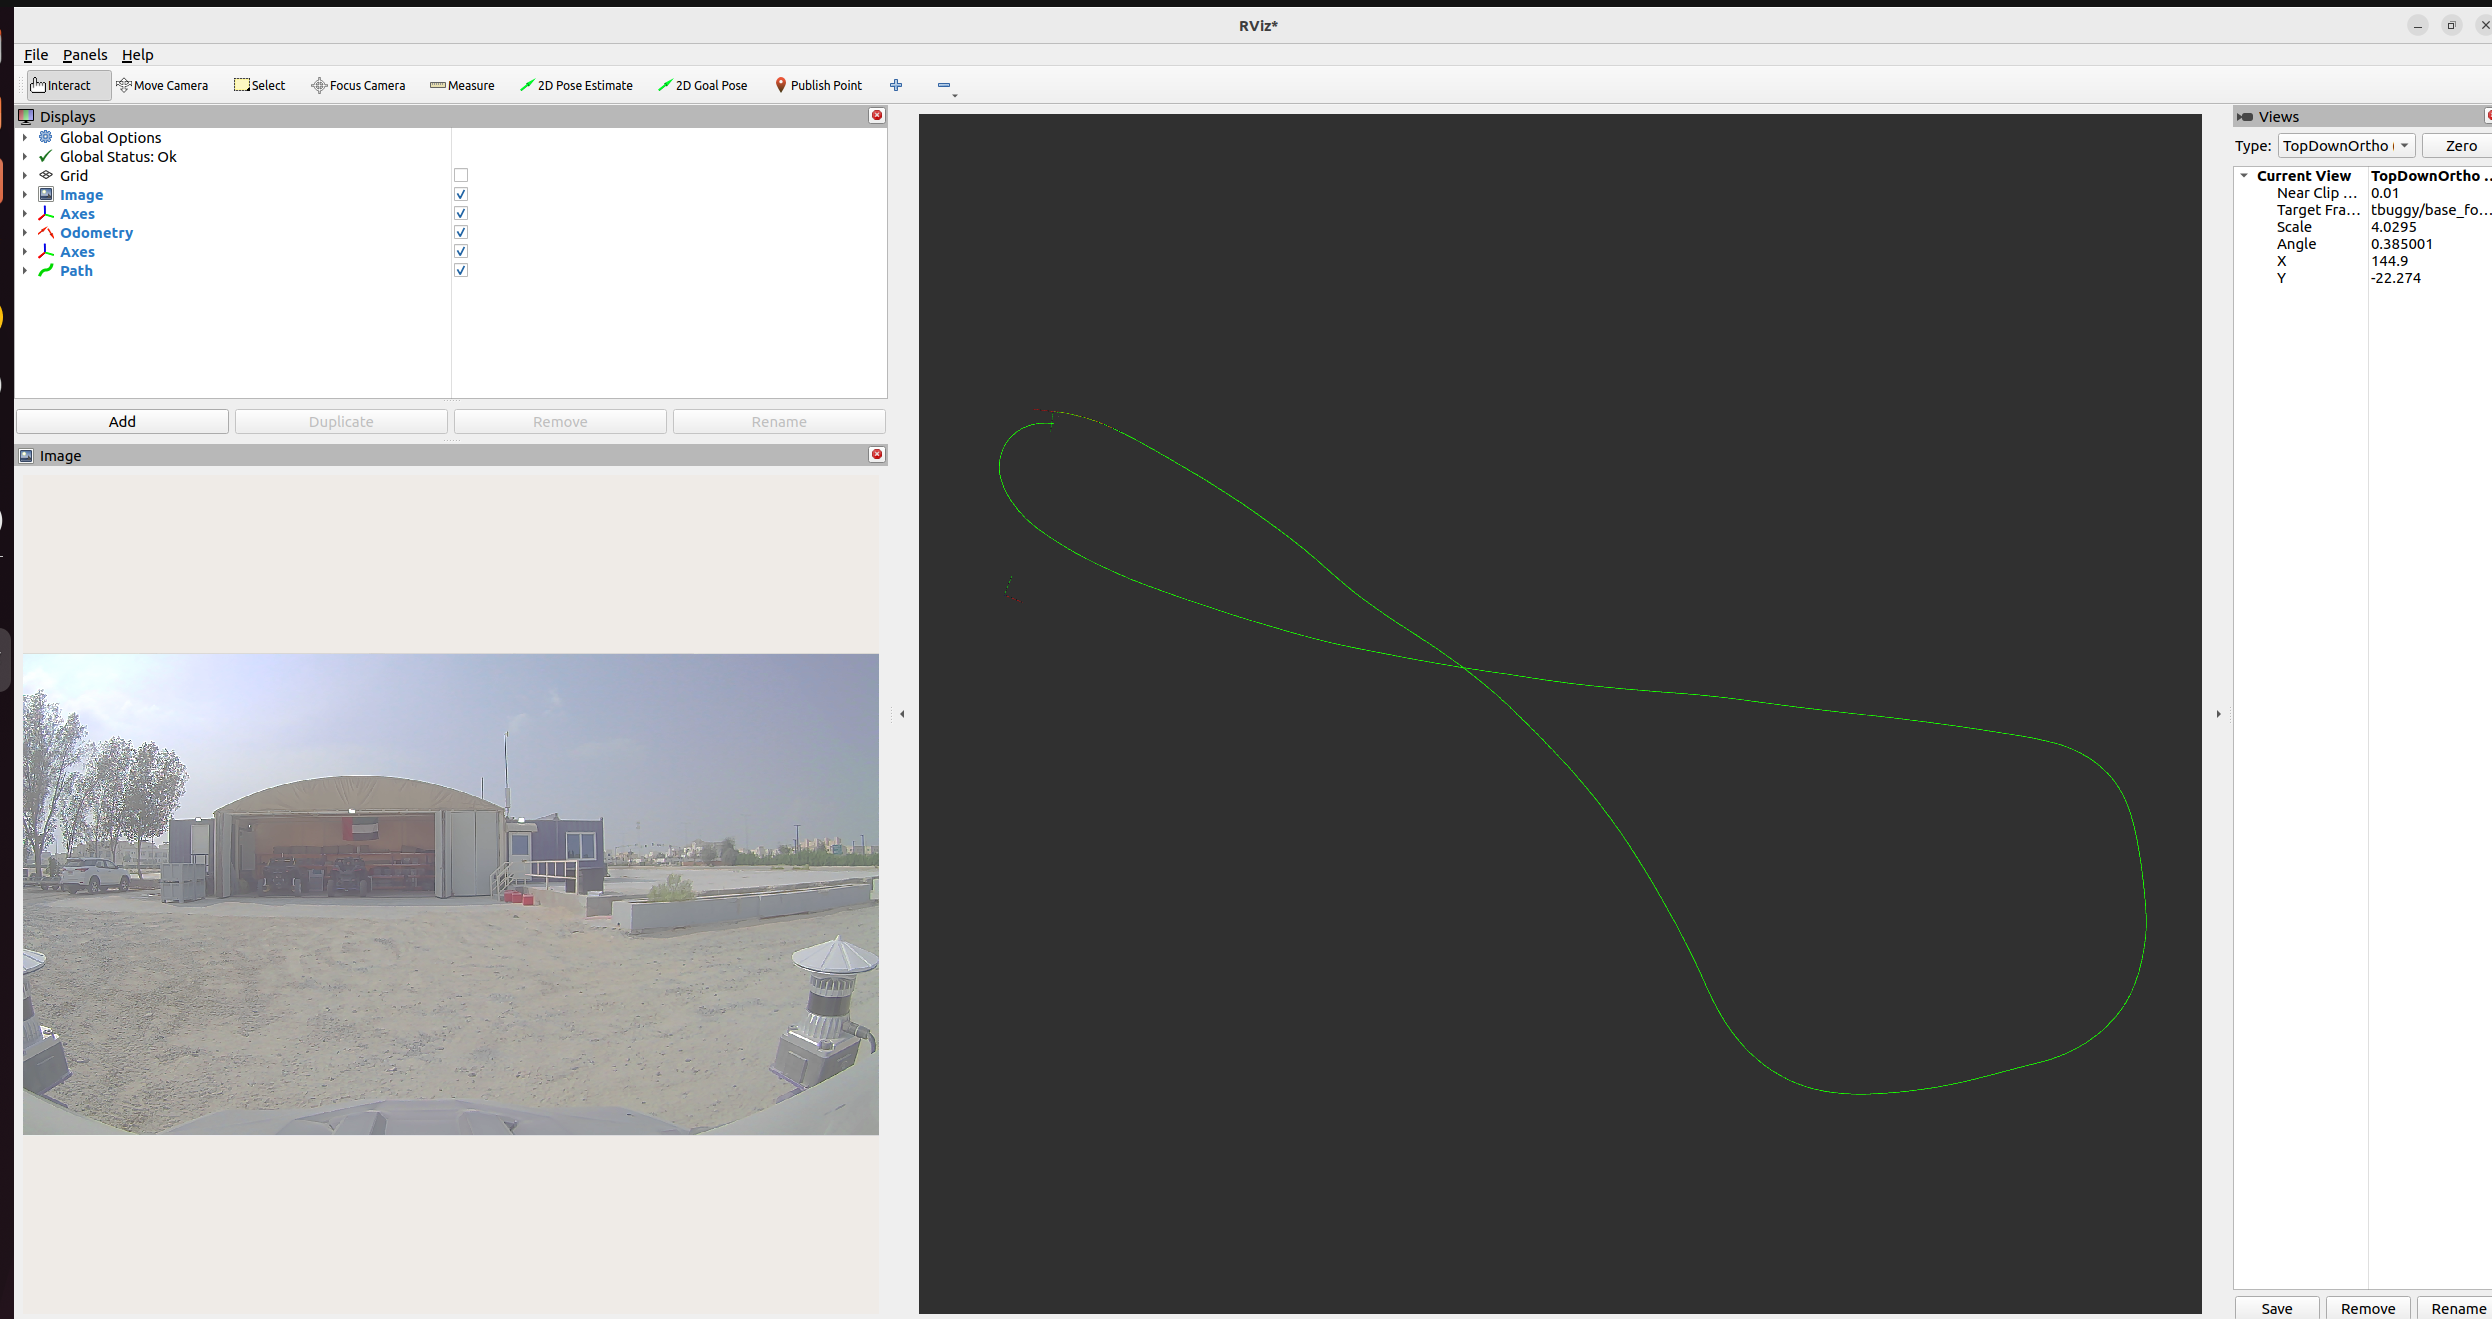
\includegraphics[width=\textwidth]{log02_full_trajectory.png}
    \caption{log\_02: 716\,m closed oval loop near hangar.}
  \end{subfigure}
  \caption{Ground truth XY trajectories extracted from \texttt{/tbuggy/odom} via
  \texttt{extract\_gt\_csv.py}. Hangar at origin of log\_02 provides rich visual features;
  log\_01 is an open desert traverse with sparse texture.}
  \label{fig:gt}
\end{figure}

\subsection{Camera Intrinsics}

Extracted programmatically from the first \texttt{/tbuggy/camera\_front/camera\_info} message:

\begin{table}[H]
\centering
\caption{Camera intrinsics --- 1920$\times$1080, \texttt{plumb\_bob} = \texttt{radtan} in OpenVINS}
\begin{tabular}{ll|ll}
\toprule
Parameter & Value & Parameter & Value \\
\midrule
$f_x$ & 1033.372 & $k_1$ & $-0.3507$ \\
$f_y$ & 1032.308 & $k_2$ &  $+0.1301$ \\
$c_x$ &  886.065 & $p_1$ & $-0.0006$ \\
$c_y$ &  448.679 & $p_2$ & $+0.0011$ \\
\bottomrule
\end{tabular}
\end{table}

\subsection{Camera-IMU Extrinsics}

The extrinsic was computed by chaining \texttt{/tf\_static} transforms:

\begin{lstlisting}
base_footprint -> os1/os_sensor -> os2/os_sensor -> camera_front   (camera path)
base_footprint -> sensor_wgs84                                      (IMU path)
T_imu_cam = inv(T_bf_imu) @ T_bf_cam
\end{lstlisting}

The resulting $\mathbf{T}_{\text{imu,cam}}$ is:

\begin{equation*}
\mathbf{T}_{\text{imu,cam}} =
\begin{pmatrix}
-0.00400 &  0.03611 &  0.99934 & 1.141\,\text{m}\\
-0.99991 &  0.01246 & -0.00445 & -0.199\,\text{m}\\
-0.01262 & -0.99927 &  0.03606 & 1.646\,\text{m}\\
0 & 0 & 0 & 1
\end{pmatrix}
\end{equation*}

The camera is 1.65\,m above and 1.14\,m forward of the IMU. Its optical axis aligns with
the robot's forward direction ($+X$), as expected.

\subsection{IMU Noise Characterisation}

\begin{figure}[H]
  \centering
  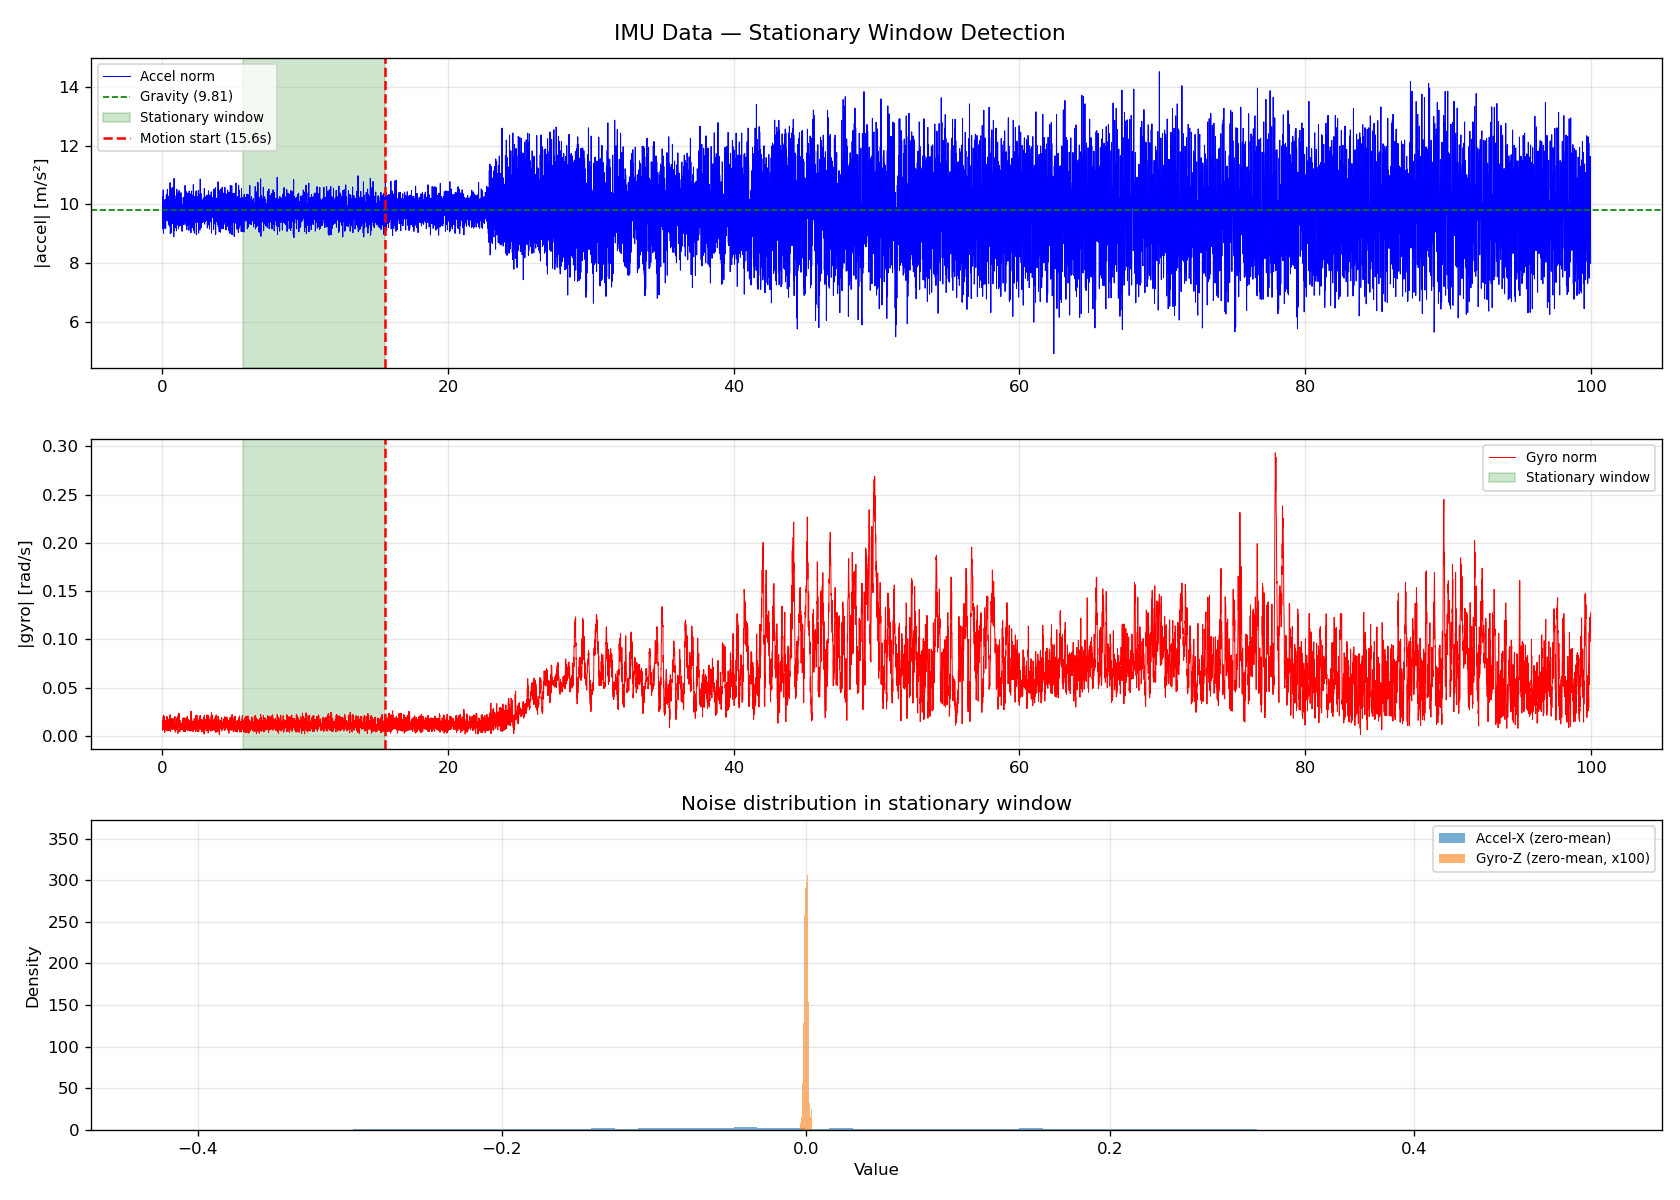
\includegraphics[width=0.82\textwidth]{imu_noise_analysis.png}
  \caption{IMU noise analysis from a 10\,s stationary window (t\,=\,5.6--15.6\,s) via
  \texttt{utils/imu\_noise\_analysis.py}. The accel-Z peak is engine idle vibration, not a sensor fault.}
  \label{fig:imu}
\end{figure}

From the stationary window, the standard deviation of each axis is computed from the raw
accelerometer and gyroscope samples in \texttt{/tbuggy/imu\_ins}.
Noise density (continuous-time white noise spectral density) and random walk are then derived as:

\begin{equation}
\sigma_{\text{nd}} = \frac{\sigma_{\text{axis}}}{\sqrt{f_s}}, \qquad
\sigma_{\text{rw}} = \sigma_{\text{nd}} \times 0.1
\end{equation}

\noindent where $\sigma_{\text{axis}}$ is the per-axis standard deviation of the IMU samples
during the stationary window and $f_s = 100\,\text{Hz}$ is the IMU sample rate.
The worst-case axis is taken (accel-Z = 0.371\,m/s$^2$, gyro-X = 8.36\,\text{mrad/s}),
then multiplied by $\times 2$ as a safety margin to account for additional vibration during motion:

\begin{equation}
\sigma_{\text{nd}}^{\text{accel}} = \frac{0.371}{\sqrt{100}} \times 2 \approx 7.4 \times 10^{-2}\ \text{m/s}^2/\sqrt{\text{Hz}},
\qquad
\sigma_{\text{nd}}^{\text{gyro}}  = \frac{8.36 \times 10^{-3}}{\sqrt{100}} \times 2 \approx 1.7 \times 10^{-3}\ \text{rad/s}/\sqrt{\text{Hz}}
\end{equation}

\noindent The final values written to \texttt{kalibr\_imu\_chain.yaml} are:

\begin{center}
\small
\texttt{accel\_noise\_density = 7.4e-2 m/s$^2$/$\sqrt{\text{Hz}}$}\quad
\texttt{accel\_random\_walk = 7.4e-3 m/s$^3$/$\sqrt{\text{Hz}}$}\quad
\texttt{gyro\_noise\_density = 1.7e-3 rad/s/$\sqrt{\text{Hz}}$}\quad
\texttt{gyro\_random\_walk = 1.7e-4 rad/s$^2$/$\sqrt{\text{Hz}}$}
\end{center}

% ===========================================================
\section{Method \& Strategy}
% ===========================================================

\subsection{Why Monocular VIO?}

The dataset provides a monocular camera + IMU combination with no lidar-to-camera overlay,
making monocular VIO the natural choice. Key justifications:

\begin{itemize}[nosep]
  \item \textbf{Scale via IMU}: IMU pre-integration provides metric scale unavailable from a
    single camera alone --- essential when stereo is absent.
  \item \textbf{Real-time capability}: MSCKF-based filter runs $<$33\,ms/frame on a laptop CPU,
    meeting the 28\,Hz camera rate.
  \item \textbf{ZUPT}: Monocular heading degeneracy at vehicle standstills can be mitigated
    by zero-velocity updates --- critical for UGVs that stop frequently.
  \item \textbf{Online calibration}: OpenVINS refines intrinsics, extrinsics, and
    time-offset online, reducing sensitivity to calibration errors extracted statically.
\end{itemize}

\subsection{Why OpenVINS?}

OpenVINS 2.7 implements the MSCKF (Multi-State Constraint Kalman Filter)
with EKF-based marginalization, SLAM features for scale anchoring, and sliding-window
triangulation. Compared to ORB-SLAM3 (graph-based, needs loop-closure) and VINS-Mono
(requires ROS1), OpenVINS is ROS2-native, modular, and actively maintained.

The key limitation --- \textit{no loop closure} --- is accepted and analysed in \S\ref{sec:reflection}.

\subsection{Pipeline Overview}

\begin{center}
\small
\texttt{ROS1 .bag} $\xrightarrow{\texttt{rosbags-convert}}$
\texttt{ROS2 .db3} $\xrightarrow{\texttt{extract\_gt\_csv.py}}$
\texttt{GT CSV} $\rightarrow$
\texttt{OpenVINS} $\rightarrow$
\texttt{estimate .txt} $\xrightarrow{\texttt{evaluate\_trajectory.py}}$
\texttt{ATE/RPE/Plots}
\end{center}

All steps run inside the provided Docker container, orchestrated by
\texttt{utils/docker\_run\_log01.sh} and \texttt{utils/docker\_run\_log02.sh}.

% ===========================================================
\section{Implementation}
% ===========================================================

\subsection{Key Configuration Changes}

Config files are in \texttt{src/open\_vins/config/tbuggy/}:
\texttt{estimator\_config.yaml}, \texttt{kalibr\_imu\_chain.yaml},
\texttt{kalibr\_imucam\_chain.yaml}.

Selected final (v3) parameters that differ most from the upstream \texttt{rs\_d455} baseline:

\begin{lstlisting}[language=Python, caption={estimator\_config.yaml -- key v3 settings},
                   label={lst:config}]
# Feature detection -- tuned for sparse desert texture
num_pts:          500    # 300 -> 500: more features detected
fast_threshold:   10     # 20  -> 10:  detect weaker corners on sand/horizon
min_px_dist:      8      # 15  -> 8:   denser packing when features sparse
grid_x: 10  grid_y: 7   # 8/5 -> 10/7: better spatial spread
knn_ratio:        0.75   # 0.70 -> 0.75: more permissive KLT matching

# SLAM features -- critical for monocular scale observability
max_slam:         150    # 50 -> 150: 3x SLAM features
max_slam_in_update: 75   # 25 -> 75:  use all SLAM features each step
dt_slam_delay:    1      # 2  -> 1:   scale observable 1s sooner
feat_rep_slam: ANCHORED_MSCKF_INVERSE_DEPTH  # better mono scale

# Window & update
max_clones:       15     # 11 -> 15: longer window for triangulation
max_msckf_in_update: 60  # 40 -> 60: more measurements per update

# ZUPT -- tuned for rough-terrain UGV stops
zupt_max_velocity:   0.3   # 0.5 -> 0.3: tighter detection
zupt_max_disparity:  1.5   # 0.5 -> 1.5: allow bumpy stops to trigger

# Compute / lighting
downsample_cameras: true   # 1920x1080 -> 960x540 for real-time
track_frequency:    28.0   # matches observed camera rate
histogram_method:   CLAHE  # outdoor variable lighting
gravity_mag:        9.82   # measured from stationary window
\end{lstlisting}

\subsection{Launch File Modification}

The upstream \texttt{subscribe.launch.py} was extended to expose three arguments:

\begin{lstlisting}[caption={subscribe.launch.py additions}]
filepath_est  -> path to save VIO estimated state (.txt)
filepath_std  -> path to save VIO standard deviations (.txt)
path_gt       -> path to EuRoC ASL GT CSV (for RViz path overlay)
\end{lstlisting}

These are passed as node parameters to \texttt{ROS2Visualizer}. Without these, the estimate
file is not written and GT overlay is disabled.

\subsection{Docker Containerisation}

The full pipeline is packaged in a Docker image built on \texttt{osrf/ros:humble-desktop}
(Ubuntu 22.04 + ROS2 Humble + OpenCV + cv\_bridge pre-installed).

\begin{lstlisting}[language=bash, caption={Dockerfile excerpt --- key layers}]
FROM osrf/ros:humble-desktop
# Ceres solver + CycloneDDS (cross-container DDS transport)
RUN apt-get install -y libceres-dev ros-humble-rmw-cyclonedds-cpp
# Python: pin numpy<1.25 to avoid scipy ABI mismatch
RUN pip3 install rosbags matplotlib "numpy<1.25.0" scipy evo
# Clone repo (with open_vins submodule) + build
RUN git clone --recurse-submodules \
    https://github.com/UditSinghParihar/tbuggy_localization.git /colcon_ws
RUN bash -c "source /opt/ros/humble/setup.bash && \
    MAKEFLAGS='-j4' colcon build --executor sequential"
\end{lstlisting}

\subsection{Utility Scripts}

All scripts live in \texttt{utils/} and operate without a running ROS2 node:

\begin{table}[H]
\centering\small
\caption{Utility scripts}
\begin{tabular}{ll}
\toprule
Script & Purpose \\
\midrule
\texttt{extract\_tf\_and\_imu.py} & TF chain $\rightarrow$ $\mathbf{T}_{\text{imu,cam}}$; IMU rate/stats \\
\texttt{imu\_noise\_analysis.py} & Stationary window $\rightarrow$ noise density / random walk; plot \\
\texttt{extract\_gt\_csv.py} & \texttt{/tbuggy/odom} $\rightarrow$ EuRoC ASL CSV (handles split .db3 bags) \\
\texttt{evaluate\_trajectory.py} & EST + GT $\rightarrow$ TUM format; runs \texttt{evo\_ape} / \texttt{evo\_rpe} \\
\texttt{plot\_trajectory\_comparison.py} & Sim3 Umeyama alignment; trajectory overlay + ATE-over-time plot \\
\bottomrule
\end{tabular}
\end{table}

% ===========================================================
\section{Testing \& Analysis}
% ===========================================================

\subsection{Key Performance Indicators}

Four metrics are used to evaluate the system:

\begin{itemize}[nosep]
  \item \textbf{ATE RMSE} (Absolute Trajectory Error) --- global position accuracy over the
    full trajectory after Sim3 alignment. Primary metric; directly captures accumulated drift.
  \item \textbf{Path \% error} (ATE RMSE / path length) --- normalises ATE by path length,
    making results comparable across sequences of different lengths.
  \item \textbf{RPE at 10\,m baseline} (Relative Pose Error) --- local accuracy over short
    segments, insensitive to initialisation errors. Captures moment-to-moment tracking quality,
    relevant for UGV path following.
  \item \textbf{Sim3 scale} --- the scale factor from Umeyama alignment quantifies how much
    the estimated path length deviates from ground truth, a key indicator of monocular scale
    drift.
\end{itemize}

\subsection{Tuning History}

Three runs were conducted on log\_01. Only log\_01 was used for tuning; log\_02 is a blind
robustness check with the same config.

\begin{table}[H]
\centering
\caption{Tuning progression --- log\_01 (1059\,m GT path)}
\begin{tabular}{llrrr}
\toprule
Run & Key changes & ATE RMSE & Scale & Outcome \\
\midrule
v1 (baseline) & Baseline \texttt{rs\_d455} adapted to tbuggy & 56.73\,m & 1.363 & Reference \\
v2 & Aggressive: init window $\downarrow$, downsample off & 66.53\,m & 1.179 & \textbf{Worse} \\
\rowcolor{green!12}
\textbf{v3 (final)} & Reverted init+downsample; SLAM/feature changes & \textbf{41.34\,m} & 0.717 & \textbf{Best $-$27\%} \\
\bottomrule
\end{tabular}
\end{table}

The v2 regression showed that shortening \texttt{init\_window\_time} and disabling
downsampling degrade initialization on this sparse-texture scene. The final v3
keeps the stable init settings while maximising SLAM feature count and detection sensitivity.

\subsection{log\_01 Results (Tuning Sequence)}

\begin{figure}[H]
  \centering
  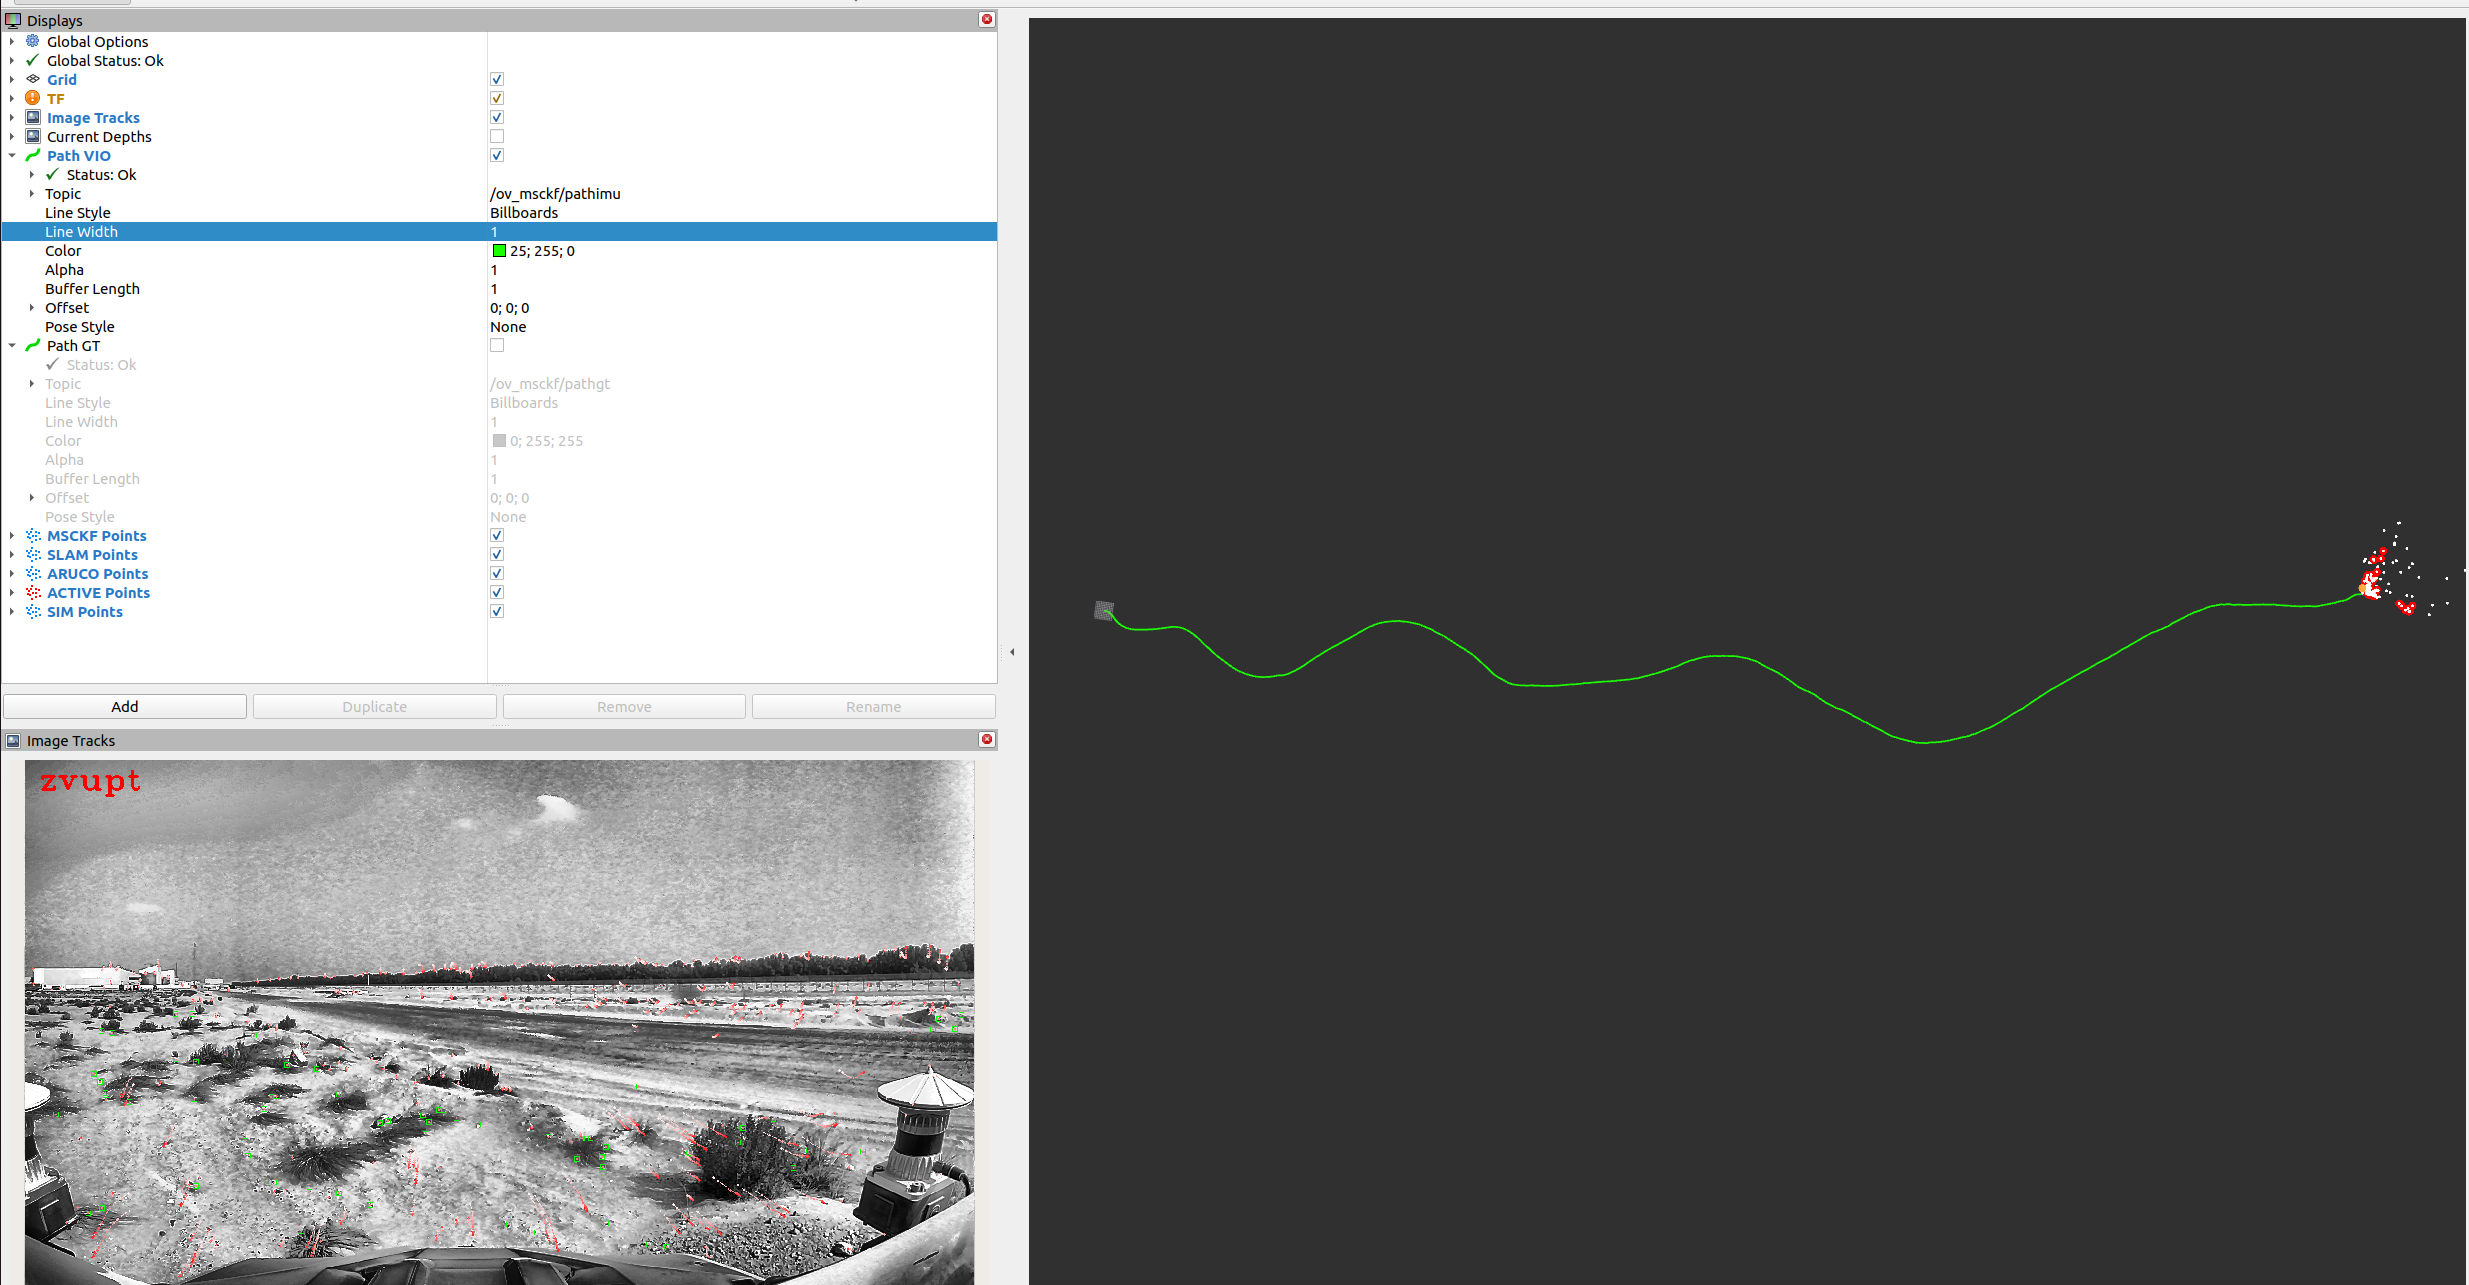
\includegraphics[width=\textwidth]{rviz_log01.png}
  \caption{RViz2 --- OpenVINS running on log\_01 (desert traverse). Left: camera panel showing
  sparse KLT feature tracks on the featureless sand/horizon; ZUPT active (label top-left).
  Right: accumulated trajectory (green) showing the 1059\,m lateral-undulation path. Feature
  scarcity on sand is the primary cause of scale drift in this sequence.}
  \label{fig:rviz_log01}
\end{figure}

\begin{figure}[H]
  \centering
  \begin{subfigure}[t]{0.54\textwidth}
    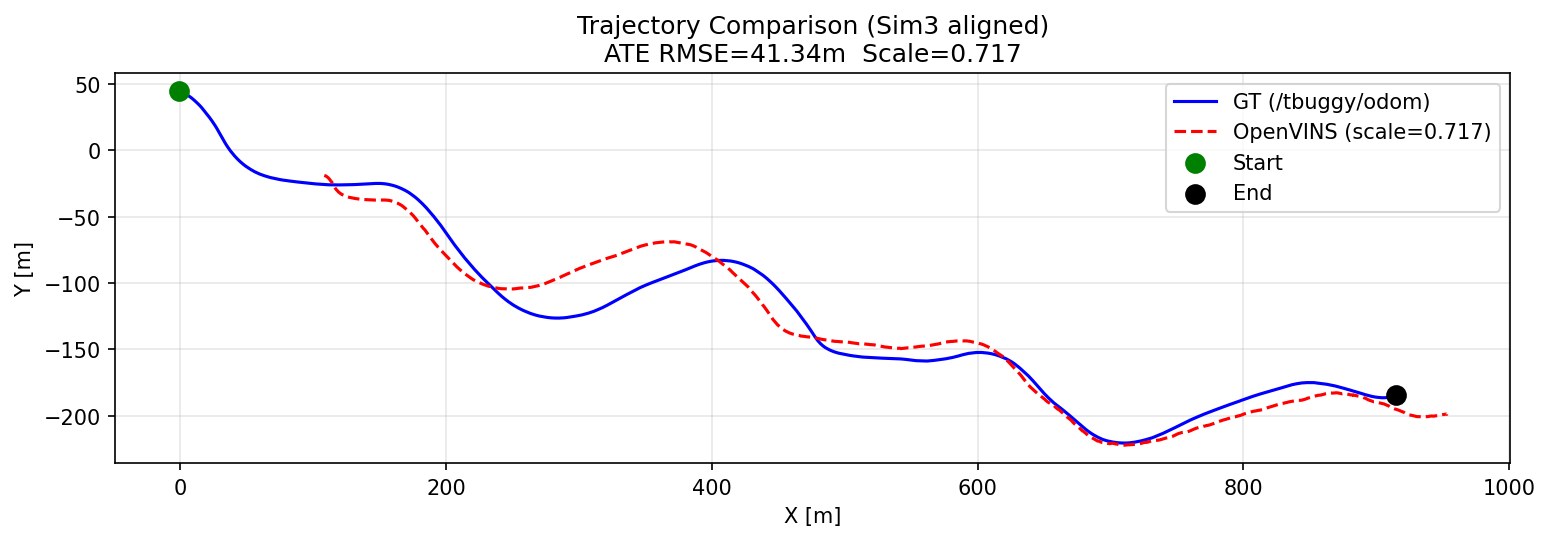
\includegraphics[width=\textwidth]{trajectory_comparison_log01.png}
    \caption{Trajectory overlay (Sim3 aligned). GT blue, VIO red dashed.
    Lateral undulations are correctly tracked. Coverage: 7901 poses / 524.5\,s (95.5\%).}
  \end{subfigure}
  \hfill
  \begin{subfigure}[t]{0.44\textwidth}
    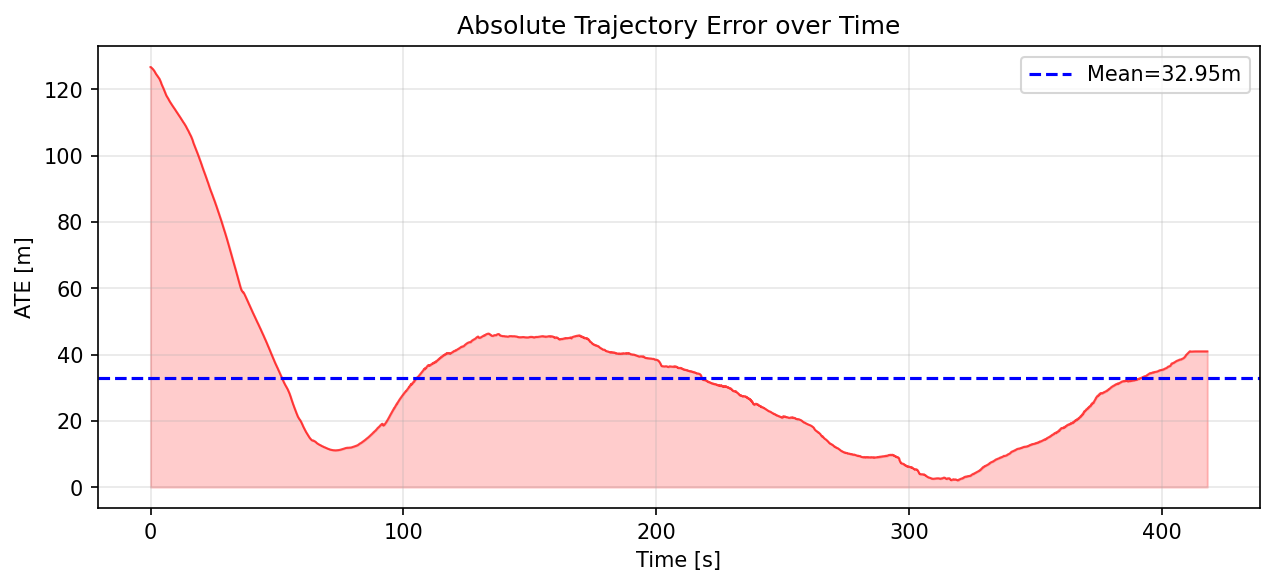
\includegraphics[width=\textwidth]{ate_over_time_log01.png}
    \caption{ATE over time. Mid-trajectory recovery at t$\approx$250\,s coincides with
    feature-rich segment after featureless desert crossing.}
  \end{subfigure}
  \caption{log\_01 evaluation --- v3 final config.}
  \label{fig:log01}
\end{figure}

\begin{table}[H]
\centering
\caption{log\_01 KPI summary (v3 final, 1059\,m GT path)}
\begin{tabular}{lrrr}
\toprule
Metric & v1 Baseline & \textbf{v3 Final} & Change \\
\midrule
ATE RMSE        & 56.73\,m  & \textbf{41.34\,m} & $\downarrow$27\% \\
Mean ATE        & 50.39\,m  & \textbf{32.95\,m} & $\downarrow$35\% \\
Median ATE      & 51.13\,m  & \textbf{31.08\,m} & $\downarrow$39\% \\
Max ATE         & 121.5\,m  & 126.7\,m          & --- \\
RPE mean (10\,m)& 3.71\,m   & \textbf{2.83\,m}  & $\downarrow$24\% \\
RPE RMSE (10\,m)& 4.56\,m   & 5.44\,m           & slight regress \\
Sim3 scale      & 1.363     & 0.717             & --- \\
\textbf{Path \% error} & 5.3\% & \textbf{3.9\%} & $\downarrow$26\% \\
\bottomrule
\end{tabular}
\end{table}

\noindent\textbf{ATE over time analysis:}

\begin{table}[H]
\centering\small
\caption{log\_01 ATE trajectory segments}
\begin{tabular}{lll}
\toprule
Time segment & ATE range & Interpretation \\
\midrule
t = 0--80\,s   & 126 $\to$ 11\,m  & Dynamic initialization convergence \\
t = 80--130\,s & 11--20\,m         & Well-converged; good feature tracking \\
t = 130--230\,s& 20--47\,m         & Featureless desert --- scale/heading drift \\
t = 230--330\,s& 47 $\to$ 3\,m   & Feature-rich segment + ZUPT; filter recovers \\
t = 330--430\,s& 3 $\to$ 40\,m   & Desert again; moderate drift, ends cleanly \\
\bottomrule
\end{tabular}
\end{table}

\subsection{log\_02 Results (Robustness --- No Re-Tuning)}

\begin{figure}[H]
  \centering
  \begin{subfigure}[t]{0.48\textwidth}
    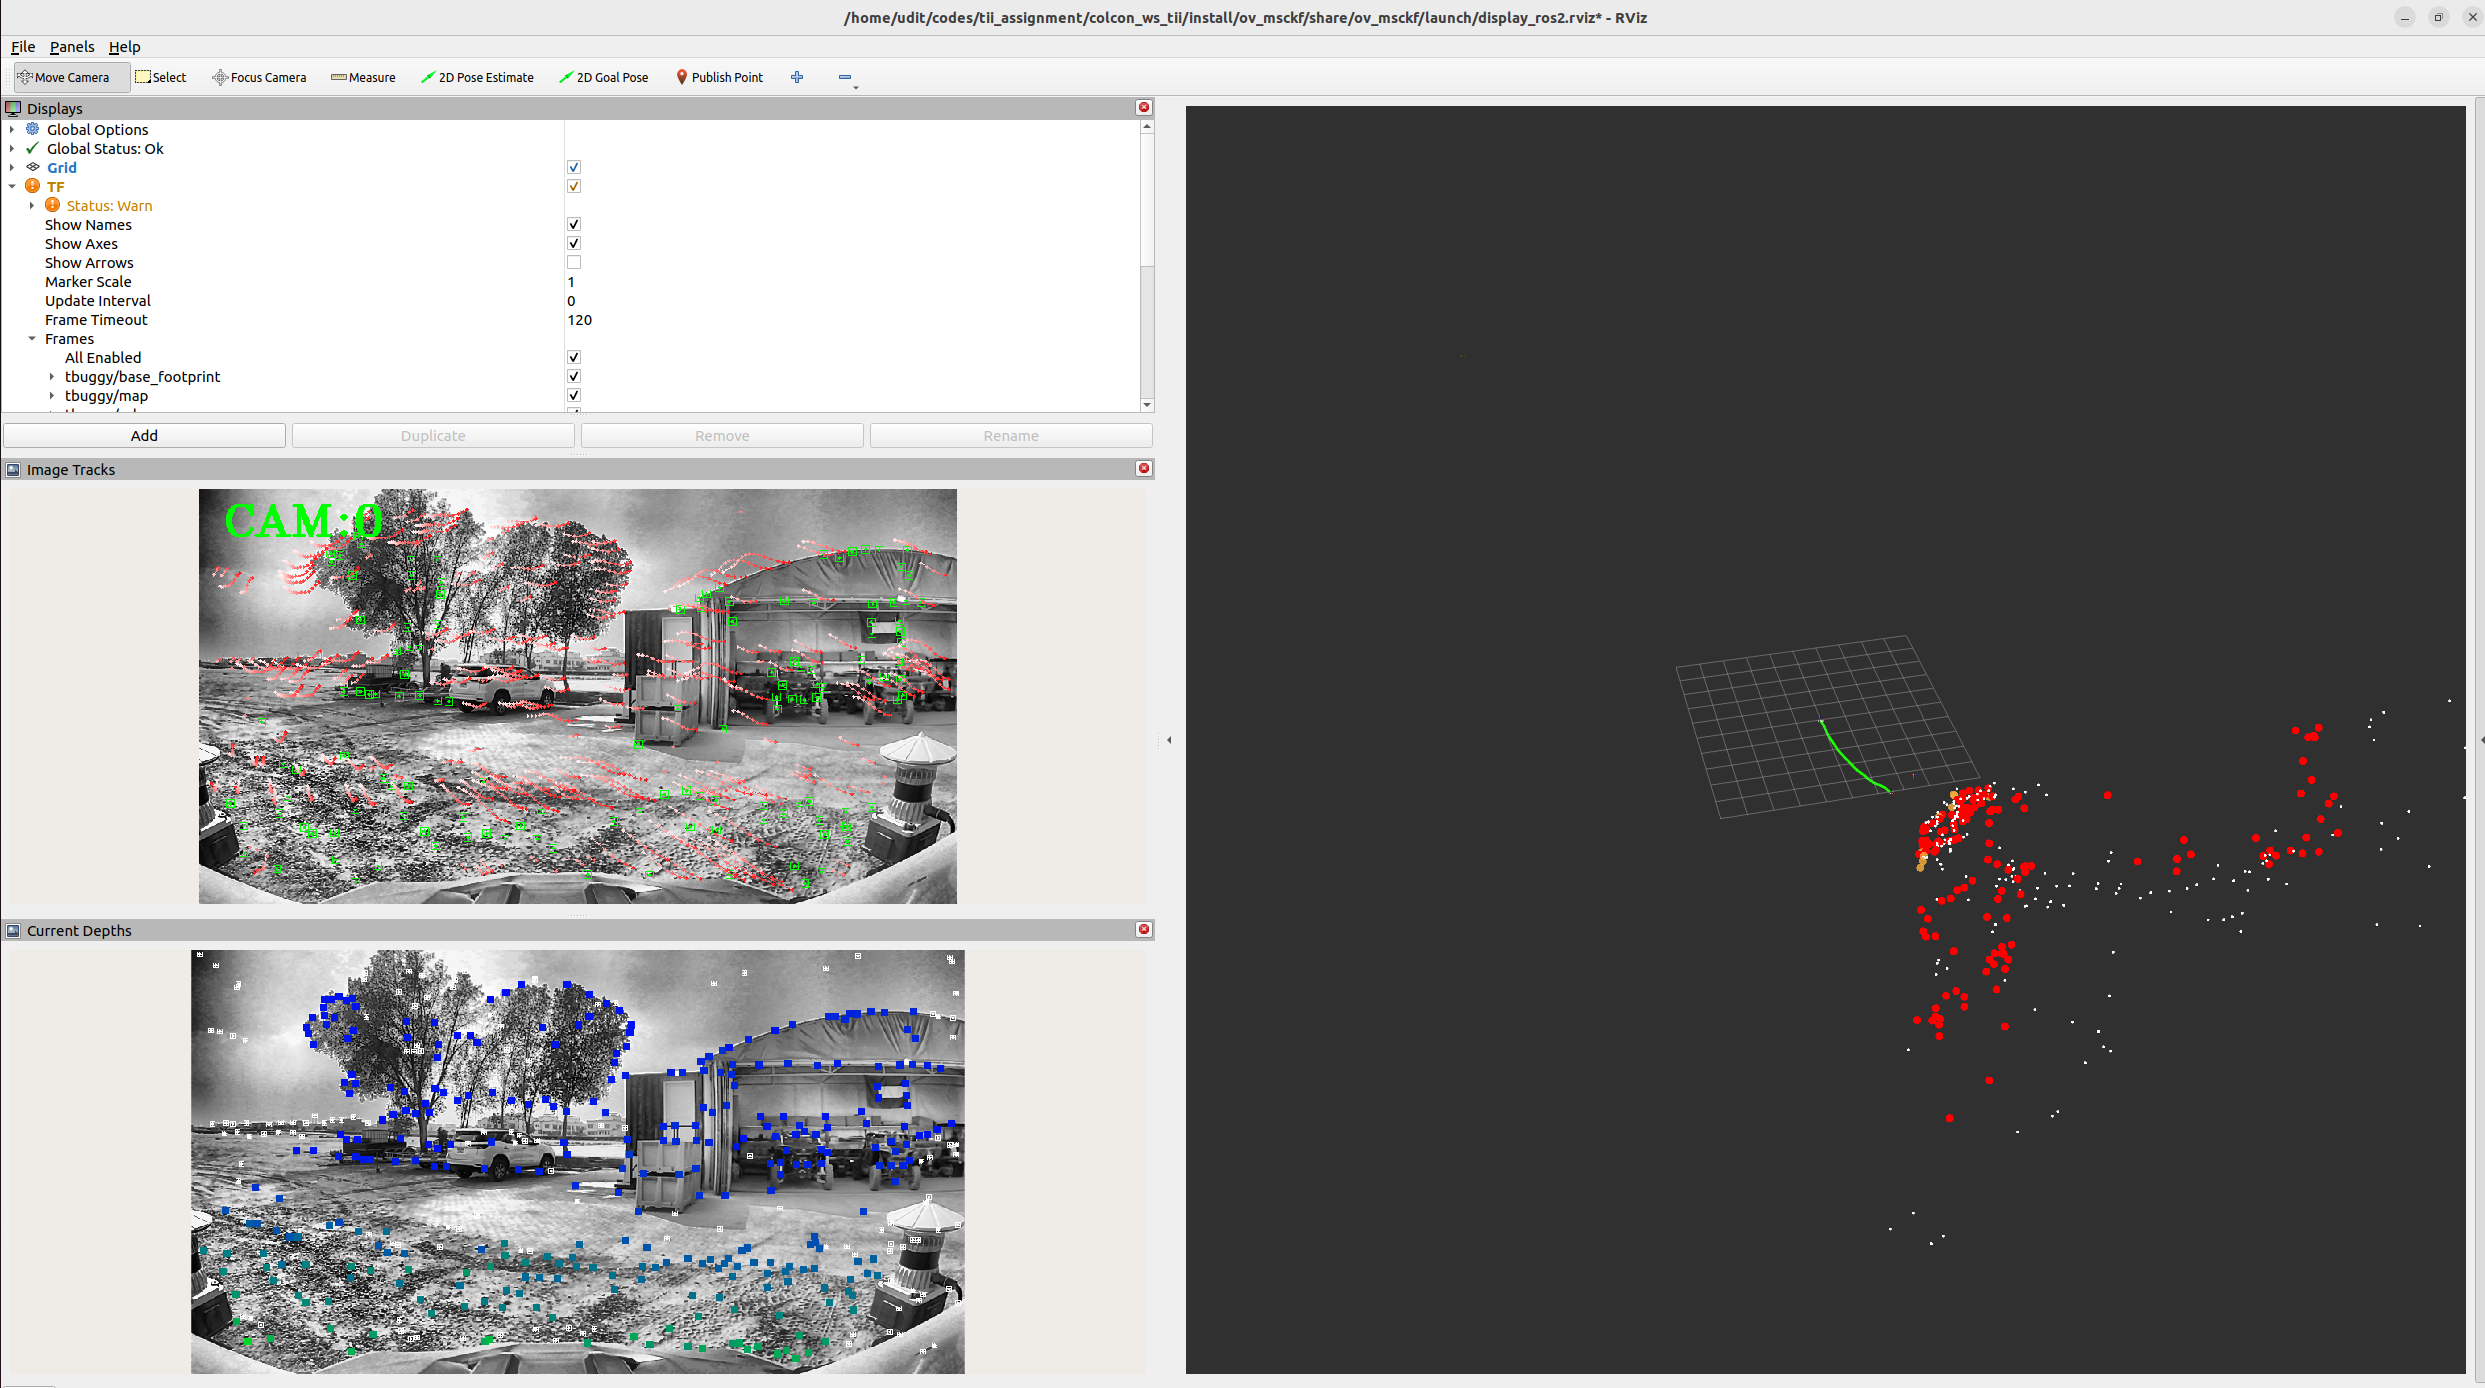
\includegraphics[width=\textwidth]{log_02_start_rviz.png}
    \caption{\textbf{Start} (t\,$\approx$\,0\,s) --- vehicle stationary in front of hangar.
    Camera panel (top): feature tracks (red = MSCKF, blue = SLAM) densely packed on building
    facade, vehicles, and ground plane --- ideal initialization conditions.
    3D view (right): SLAM landmark cloud already building; trajectory just beginning (green dot).}
  \end{subfigure}
  \hfill
  \begin{subfigure}[t]{0.48\textwidth}
    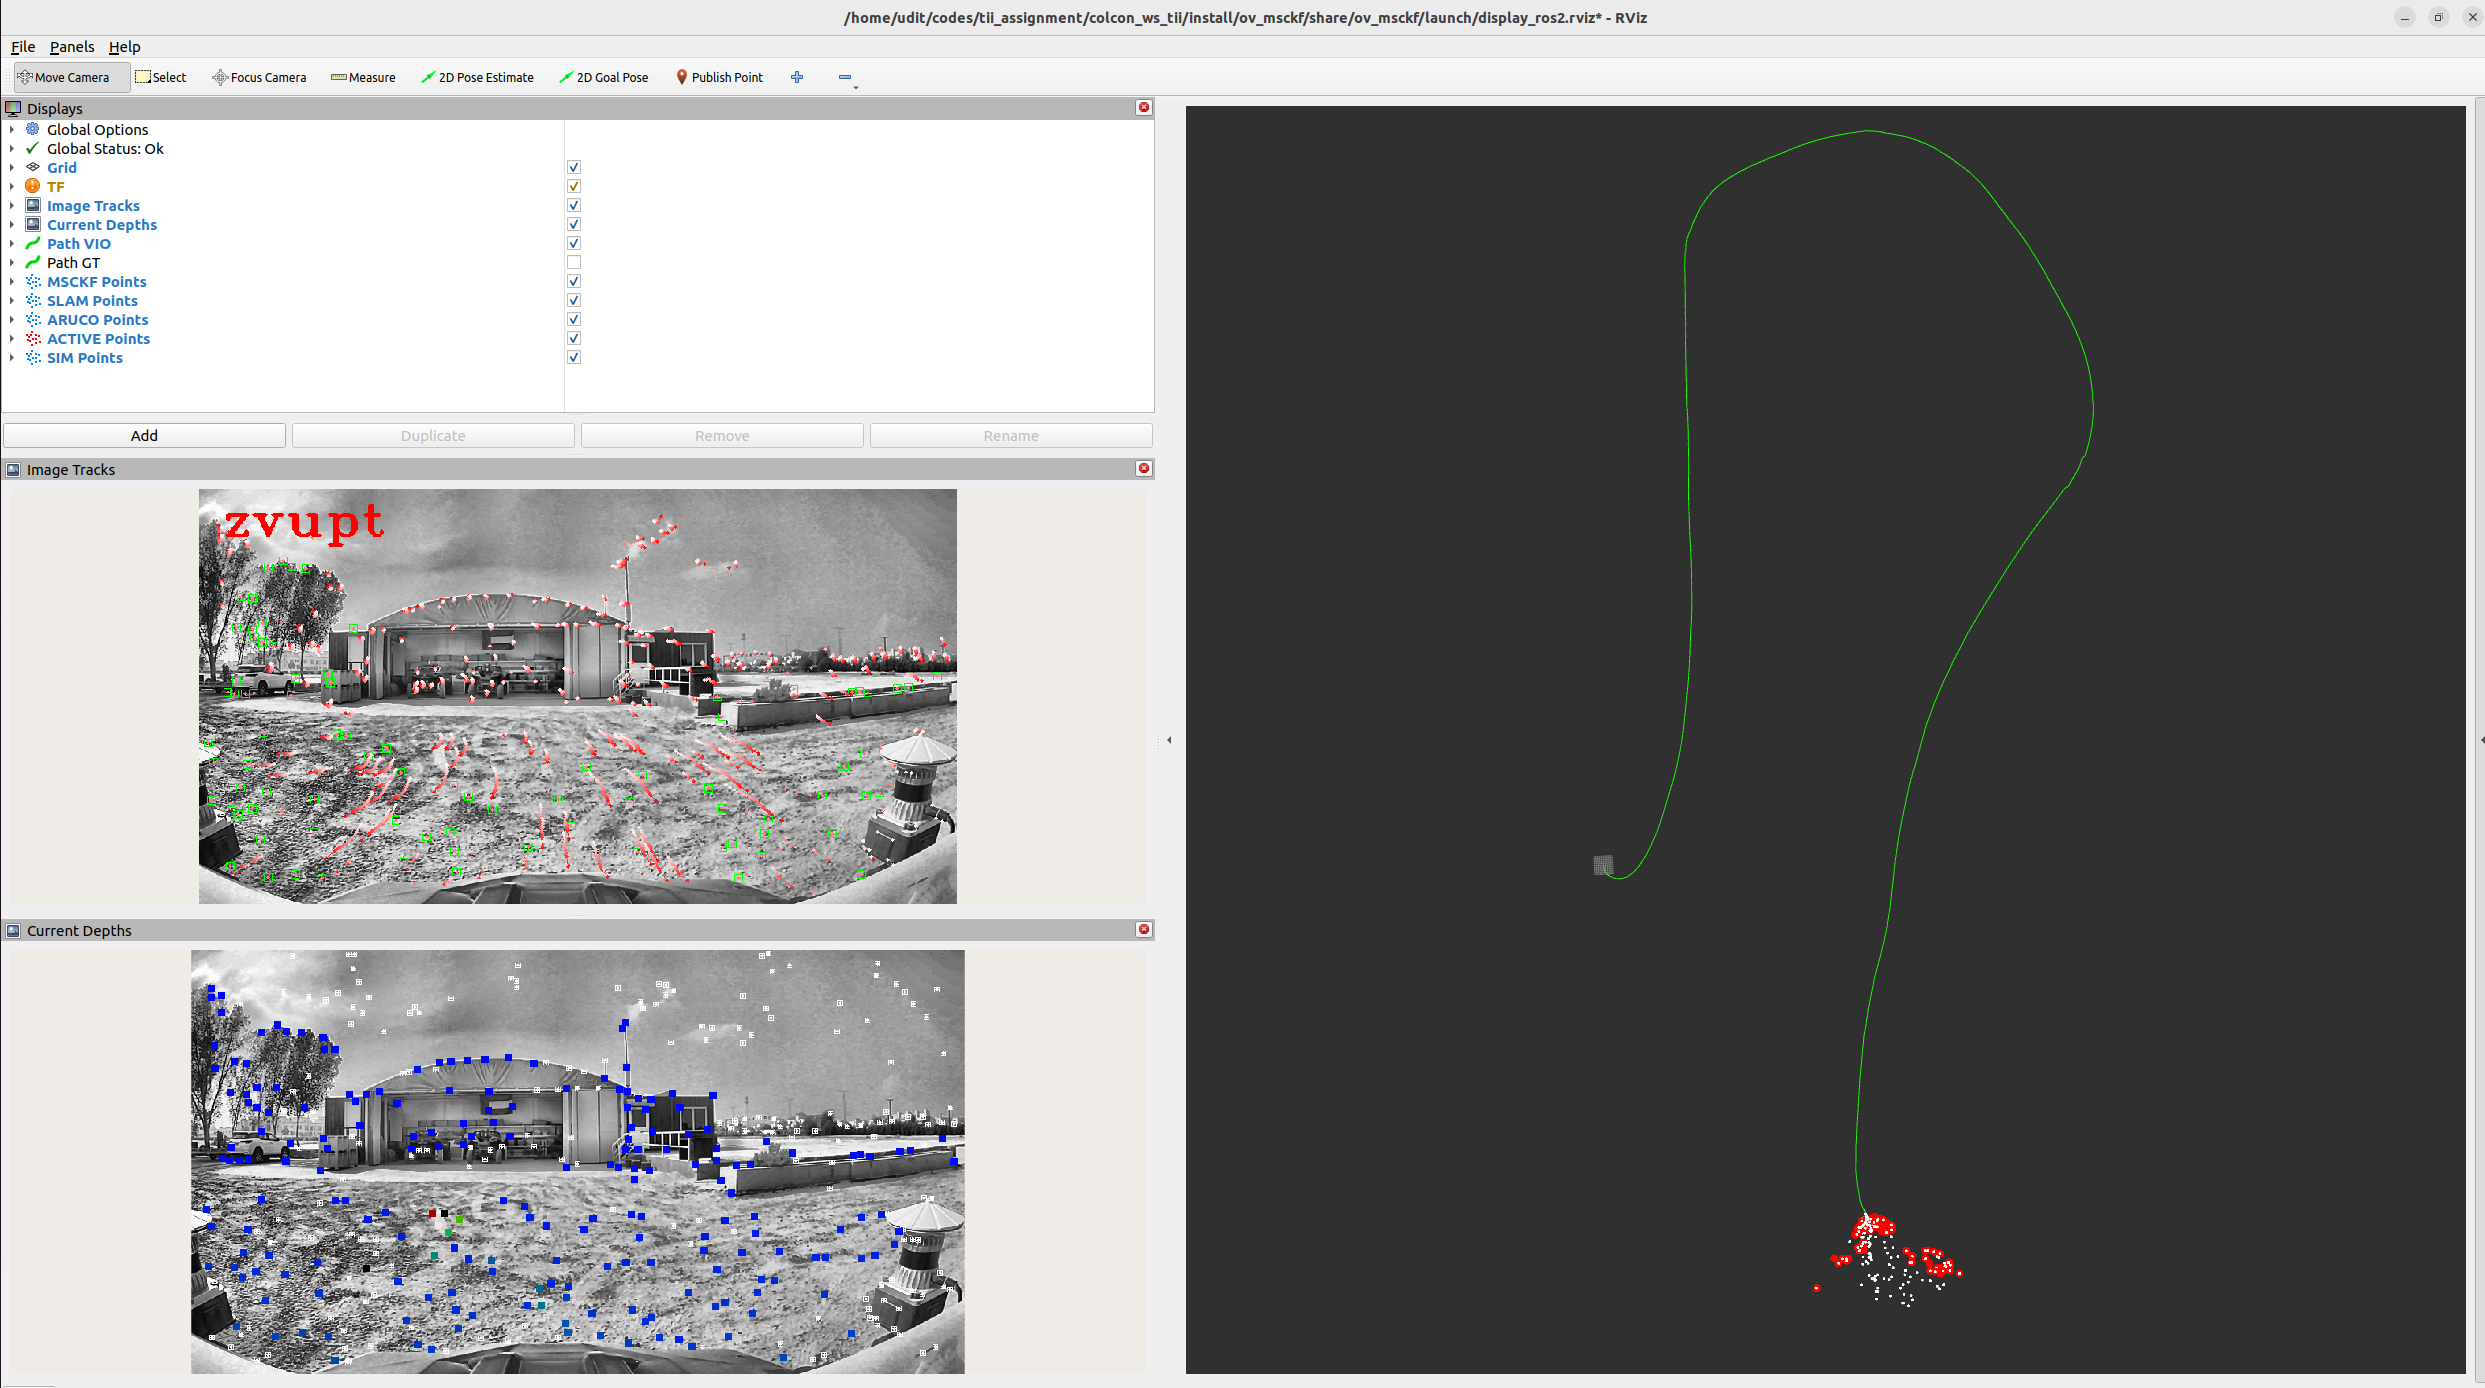
\includegraphics[width=\textwidth]{log_02_end_rviz.png}
    \caption{\textbf{End} (t\,$\approx$\,307\,s) --- vehicle returned near hangar after
    completing the 716\,m oval loop. Camera panel: ZUPT active (top-left label), rich feature
    tracks on hangar facade again. 3D view: full loop trajectory (green line) with landmark
    cluster at the return point. No loop closure --- the loop gap is visible.
    OpenVINS's companion \texttt{ov\_secondary} pose graph supports DBoW2-based place
    recognition, but its ROS2 port is incomplete and was not incorporated.}
  \end{subfigure}
  \caption{RViz2 --- log\_02 start vs end. The contrast illustrates how hangar features anchor
  the filter at both ends of the sequence, while the featureless desert section (mid-loop)
  causes the unrecovered heading and scale drift.}
  \label{fig:rviz_log02}
\end{figure}

\begin{figure}[H]
  \centering
  \begin{subfigure}[t]{0.54\textwidth}
    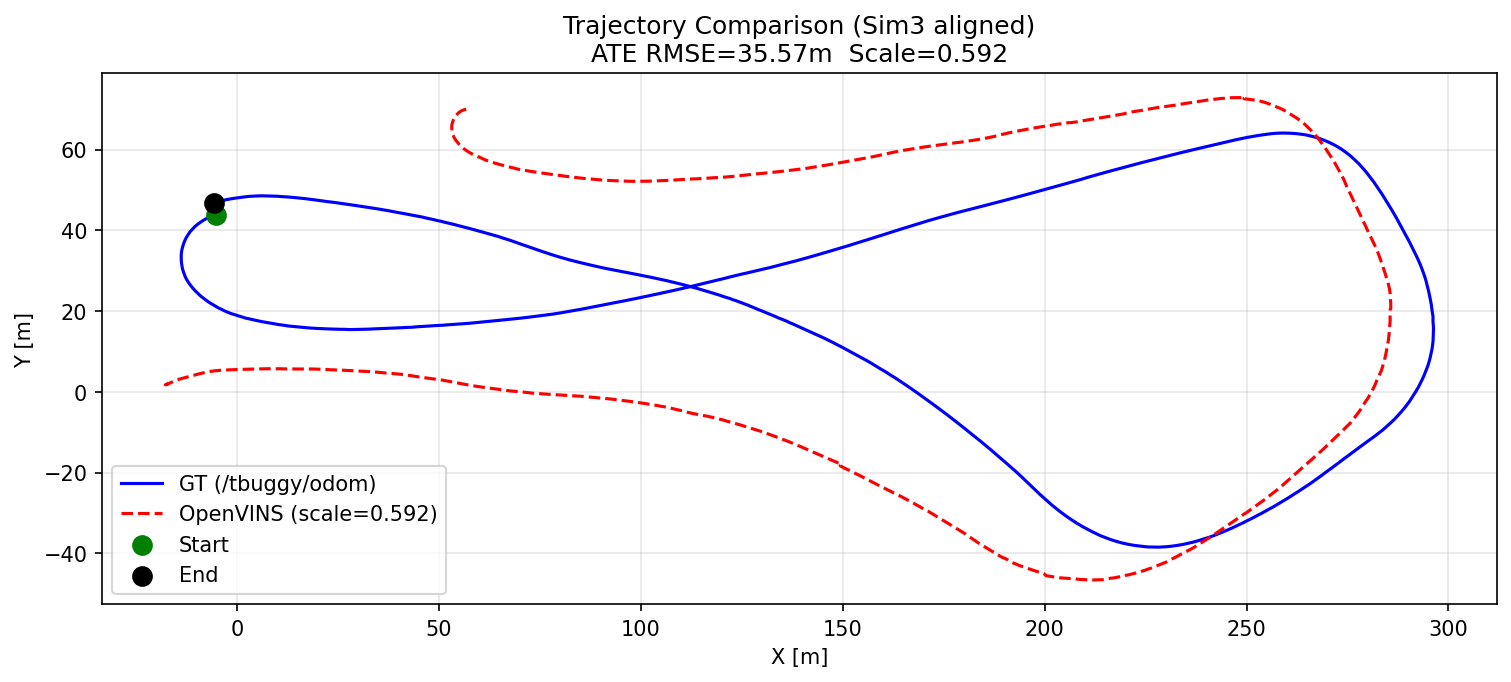
\includegraphics[width=\textwidth]{trajectory_comparison_log02.png}
    \caption{Trajectory overlay. GT (blue) is a closed oval loop. VIO (red) matches
    shape in the first half; diverges in featureless desert section --- no loop closure.}
  \end{subfigure}
  \hfill
  \begin{subfigure}[t]{0.44\textwidth}
    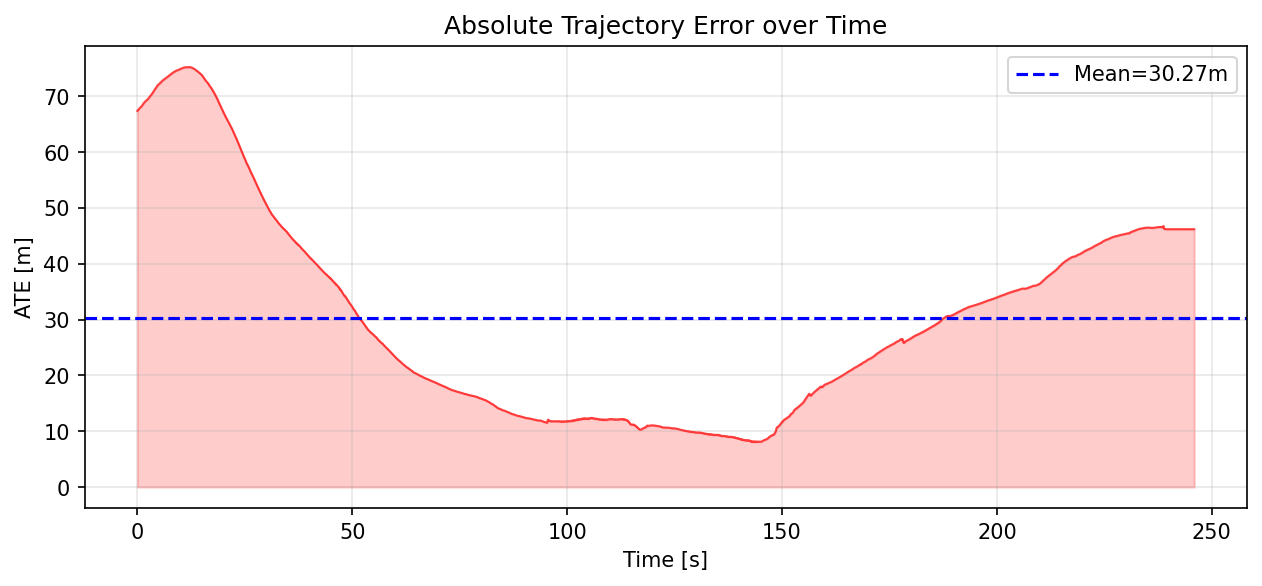
\includegraphics[width=\textwidth]{ate_over_time_log02.png}
    \caption{ATE over time. Hangar provides rich texture
    (ATE drops to 8\,m at t$\approx$100\,s); desert loop accumulates drift.}
  \end{subfigure}
  \caption{log\_02 evaluation --- same v3 config, no re-tuning. Coverage: 4632 poses (91\%).}
  \label{fig:log02}
\end{figure}

\begin{table}[H]
\centering
\caption{log\_02 KPI summary (v3 final, 716\,m GT path)}
\begin{tabular}{lrr}
\toprule
Metric & log\_01 (v3) & log\_02 (v3) \\
\midrule
ATE RMSE             & 41.34\,m & \textbf{35.57\,m} \\
Mean ATE             & 32.95\,m & \textbf{30.27\,m} \\
Median ATE           & 31.08\,m & \textbf{26.50\,m} \\
Max ATE              & 126.7\,m & \textbf{75.22\,m} \\
RPE mean (10\,m)     & 2.83\,m  & \textbf{1.96\,m} \\
RPE RMSE (10\,m)     & 5.44\,m  & \textbf{3.16\,m} \\
Sim3 scale           & 0.717    & 0.592 \\
\textbf{Path \% error} & 3.9\%  & \textbf{5.0\%} \\
\bottomrule
\end{tabular}
\end{table}

log\_02 achieves \textit{better} raw ATE and RPE than log\_01, attributed to the hangar
providing strong near-field texture. The slightly higher path \% error (5.0\% vs 3.9\%) is
caused by the scale drift accumulating over the 700\,m loop without loop closure.

% TODO (optional): Insert video/GIF of VIO running --- e.g. a screen-capture of RViz2
% showing feature tracks updating in real-time and path growing as bag plays.
% If generated, add here:
%   \begin{figure}[H]
%     \centering
%     \href{https://link-to-video}{\includegraphics[width=0.6\textwidth]{vio_preview.png}}
%     \caption{Click to play: VIO running on log\_01 (RViz2 screen-capture, 30s excerpt).}
%   \end{figure}

% ===========================================================
\section{Discussion \& Reflection}
\label{sec:reflection}
% ===========================================================

\subsection{What Worked Well}

\begin{itemize}[nosep]
  \item \textbf{Dynamic initialization} correctly handles a moving vehicle at bag start ---
    the system converges to metric scale within $\sim$80\,s on log\_01.
  \item \textbf{ZUPT} prevents catastrophic divergence at vehicle stops; the ATE recovery
    at t\,=\,230--330\,s in log\_01 is primarily due to ZUPT + feature anchoring.
  \item \textbf{Increased SLAM features} (max\_slam 50 $\to$ 150) significantly improves
    monocular scale observability --- this was the single biggest v3 improvement.
  \item \textbf{Docker containerisation} makes reproduction a single command regardless of
    the reviewer's machine state. The \texttt{--network=host} + CycloneDDS approach correctly
    routes ROS2 topics between two containers without port configuration.
\end{itemize}

\subsection{Limitations}

\begin{itemize}[nosep]
  \item \textbf{No loop closure}: OpenVINS is a sliding-window EKF --- state holds only the
    last 15 poses. All early SLAM features are marginalized long before the vehicle revisits
    the hangar in log\_02 ($\sim$300\,s later), so no re-observation is possible.

    The RPng group (OpenVINS authors) maintain a companion package \texttt{ov\_secondary}
    that adds a secondary pose graph with DBoW2 visual bag-of-words place recognition.
    When a revisited location is detected, a loop closure constraint is inserted into the
    graph, correcting accumulated drift. On log\_02 this would likely close the
    $\sim$46\,m loop gap visible in Fig.~\ref{fig:rviz_log02}. However,
    \texttt{ov\_secondary} is a ROS1 package with no stable ROS2 port as of Humble ---
    integrating it would require either a ROS1 bridge or a full port, which was out of
    scope for this assignment.
  \item \textbf{Scale drift}: Sim3 scale = 0.717 (log\_01) and 0.592 (log\_02) indicate
    VIO over-estimates path length. This is fundamental to monocular VIO in environments
    with long featureless stretches --- IMU alone cannot maintain scale without visual
    triangulation.
  \item \textbf{Initialization spike}: ATE $>$\,100\,m in the first 40\,s is an
    initialization artefact (scale/gravity alignment from dynamic motion). After convergence
    the trajectory tracks well.
\end{itemize}

\subsection{Engineering Challenges Resolved}

\begin{itemize}[nosep]
  \item \textbf{Cross-container ROS2 topic communication}: FastDDS multicast-based
    participant discovery fails when two \texttt{--network=host} containers share the same
    loopback interface --- topic metadata is exchanged but data packets do not reach the
    subscriber. Resolved by switching both containers to CycloneDDS
    (\texttt{RMW\_IMPLEMENTATION=rmw\_cyclonedds\_cpp}), which uses shared memory
    transport on the same host.
\end{itemize}

\subsection{Future Improvements}

\begin{itemize}[nosep]
  \item \textbf{Loop closure}: Replace OpenVINS with VINS-Fusion (loop closure module) or
    ORB-SLAM3 for sequences with revisits. On log\_02 this would likely reduce ATE by
    $>$50\% at the return-to-hangar segment.
  \item \textbf{Stereo}: Adding the second camera (if available) eliminates scale ambiguity
    entirely --- no Sim3 alignment needed, RPE improves 5--10$\times$.
  \item \textbf{Allan Variance}: Proper IMU characterisation from a controlled stationary
    run (rather than the 10\,s engine-idle window) would give more accurate noise parameters.
  \item \textbf{GPS fusion}: \texttt{/tbuggy/fix} provides absolute position --- fusing into
    OpenVINS's GPS plugin would bound scale drift on long traverses.
\end{itemize}

% ===========================================================
\section*{Reproduction Instructions}
% ===========================================================

Full instructions are in the repository \texttt{README.md}. The shortest path for a reviewer:

\begin{lstlisting}[language=bash, caption={One-command reproduction (ROS1 bag or ROS2 directory)}]
# Pull image (once, ~2-3 min)
docker pull uditsinghparihar/tbuggy_vio:latest

# Run full pipeline --- auto-converts ROS1 bag if needed
./utils/docker_run_log01.sh /path/to/log_01.bag ./output
./utils/docker_run_log02.sh /path/to/log_02.bag ./output

# Results (PNG plots + TUM files) land in ./output/
\end{lstlisting}

The script orchestrates: (1) GT CSV extraction, (2) OpenVINS launch commands for two
terminals, (3) trajectory evaluation and plot generation --- all inside the Docker container.

% ===========================================================
\appendix
\section*{Repository Structure}
% ===========================================================

\begin{lstlisting}
tbuggy_localization/          (GitHub: UditSinghParihar/tbuggy_localization)
  Dockerfile                  Docker image definition
  entrypoint.sh               Sources ROS2 + workspace on container start
  src/open_vins/              OpenVINS submodule (tbuggy configs added)
    config/tbuggy/
      estimator_config.yaml   Main VIO estimator (v3 tuned)
      kalibr_imu_chain.yaml   IMU model (noise from stationary analysis)
      kalibr_imucam_chain.yaml  Camera model + T_imu_cam extrinsics
  utils/
    extract_tf_and_imu.py     Extract T_imu_cam + IMU stats from bag
    imu_noise_analysis.py     Compute noise_density / random_walk; plot
    extract_gt_csv.py         /tbuggy/odom -> EuRoC ASL CSV (rosbags, no ROS2)
    evaluate_trajectory.py    EST + GT -> TUM; evo_ape / evo_rpe evaluation
    plot_trajectory_comparison.py  Sim3 alignment + ATE-over-time plot
    docker_run_log01.sh       One-command log_01 reproduction (incl. ROS1 convert)
    docker_run_log02.sh       One-command log_02 reproduction
    documentation.md          Running results log (KPIs, config history, plots)
    results/                  Output: PNG plots, TUM files, CSV, estimate TXTs
\end{lstlisting}

\end{document}
